%% RiSE Latex Template - version 0.5
%%
%% RiSE's latex template for thesis and dissertations
%% http://risetemplate.sourceforge.net
%%
%% (c) 2012 Yguaratã Cerqueira Cavalcanti (yguarata@gmail.com)
%%          Vinicius Cardoso Garcia (vinicius.garcia@gmail.com)
%%
%% This document was initially based on UFPEThesis template, from Paulo Gustavo
%% S. Fonseca.
%%
%% ACKNOWLEDGEMENTS
%%
%% We would like to thanks the RiSE's researchers community, the 
%% students from Federal University of Pernambuco, and other users that have
%% been contributing to this projects with comments and patches.
%%
%% GENERAL INSTRUCTIONS
%%
%% We strongly recommend you to compile your documents using pdflatex command.
%% It is also recommend use the texlipse plugin for Eclipse to edit your documents.
%%
%% Options for \documentclass command:
%%         * Idiom
%%           pt   - Portguese (default)
%%           en   - English
%%
%%         * Text type
%%           bsc  - B.Sc. Thesis
%%           msc  - M.Sc. Thesis (default)
%%           qual - PHD qualification (not tested yet)
%%           prop - PHD proposal (not tested yet)
%%           phd  - PHD thesis
%%
%%         * Media
%%           scr  - to eletronic version (PDF) / see the users guide
%%
%%         * Pagination
%%           oneside - unique face press
%%           twoside - two faces press
%%
%%		   * Line spacing
%%           singlespacing  - the same as using \linespread{1}
%%           onehalfspacing - the same as using \linespread{1.3}
%%           doublespacing  - the same as using \linespread{1.6}
%%
%% Reference commands. Use the following commands to make references in your
%% text:
%%          \figref  -- for Figure reference
%%          \tabref  -- for Table reference
%%          \eqnref  -- for equation reference
%%          \chapref -- for chapter reference
%%          \secref  -- for section reference
%%          \appref  -- for appendix reference
%%          \axiref  -- for axiom reference
%%          \conjref -- for conjecture reference
%%          \defref  -- for definition reference
%%          \lemref  -- for lemma reference
%%          \theoref -- for theorem reference
%%          \corref  -- for corollary reference
%%          \propref -- for proprosition reference
%%          \pgref   -- for page reference
%%4
%%          Example: See \chapref{chap:introduction}. It will produce 
%%                   'See Chapter 1', in case of English language.

\documentclass[pt,twoside,onehalfspacing,bsc]{risethesis}

\usepackage{natbib}
\usepackage{babel}
\usepackage{supertabular}
\usepackage{microtype}
\usepackage{lscape}
\usepackage{multirow}
\usepackage{tikz}
\usepackage{float}
\usepackage{url}
\usepackage{enumitem}

%% Aumenta a margem entre o label e as tabelas
% \usepackage{caption}
% \captionsetup[table]{skip=8pt}

%% Label at the bottom
\lstset{
	captionpos=b
}

%% Change the following pdf author attribute name to your name.
\usepackage[linkcolor=blue,citecolor=blue,urlcolor=blue,colorlinks,pdfpagelabels,pdftitle={Monografia de Victor Tavares},pdfauthor={Victor Tavares}]{hyperref}

\address{SALVADOR}

\universitypt{Universidade Federal da Bahia}

\departmentpt{Departamento de Ci\^{e}ncia da Computa\c{c}\~{a}o}

\programpt{}

\majorfieldpt{Ci\^{e}ncia da Computa\c{c}\~{a}o}
\majorfielden{Computer Science}

\title{SafeWatch: Sistema de Detecção de Quedas para Smartwatches}
\date{Outubro/2016}

\author{Victor de Souza Tavares}
\adviser{Vaninha Vieira}

\begin{document}

\frontmatter
\frontpage
\presentationpage

\begin{dedicatory}
Dedico esta dissertação à minha família, amigos e professores que me deram todo o apoio necessário para chegar até aqui.
\end{dedicatory}

\begin{epigraph}[]{John Woods}
Always code as if the guy who ends up maintaining your code will be a violent psychopath who knows where you live
\end{epigraph}

\resumo
% Escreva seu resumo no arquivo resumo.tex
Quedas podem ter sérias consequências, a ponto de serem consideradas um grave problema de saúde pública que afeta principalmente a população idosa, onde está relacionado com a perda de confiança, autoestima, e autonomia. Esse problema se mostra ainda mais relevante se consideramos o crescente número de idosos que em busca de sua independência e autonomia decidem morar sozinhos. É crucial que o idoso tenha rápido acesso ao atendimento médico, parte importante para a sua rápida recuperação. A demora no atendimento médico está ligado ao aumento de taxas de mortalidade e gravidade em um evento de queda. 

Pensando nisso, foi desenvolvido o \textit{SafeWatch}, um sistema de detecção de quedas embarcado em relógios inteligentes (em inglês, Smartwatch). O sistema proposto irá monitorar o idoso através de sensores presentes no smartwatch, e ao detectar uma queda, além de vibrar no pulso do usuário, irá informar para uma lista de contatos de emergência do usuário a sua localização e a possibilidade do idoso estar em uma situação de perigo. Experimentos foram realizados com oito indivíduos de biótipos distintos, onde cada um deles deveria simular uma queda em sentidos distintos. Através deste experimento, foi possível detectar o grau de confiabilidade da aplicação utilizando os valores de \textit{Sensibilidade} e \textit{Especificidade} que atingiram 89.06\% e 100\% respectivamente.




\begin{keywords}
	Relógios Inteligentes, Computação Ubíqua, Queda, Idoso
\end{keywords}

\abstract
% Write your abstract in a file called abstract.tex
Falls is a serious problem of public health that affects mainly the elderly population, in which is related to the loss of confidence, self-esteem and autonomy. This problem is shown even more relevant if we consider the growing number of elderly, who in the search of their independence and autonomy decides to live alone. Thinking about it, the \textit{SafeWatch} was developed as a fall detection systems embedded in smartwatches already in the market. The proposed system will monitor the elderly through sensors present in the smartwatch, and when it detects a fall, it will  vibrates on the user's wrist and report to a list of emergency contacts the location and the possibility of the elderly to be in a dangerous situation. According to the experiments, it was possible to evaluate the application reliability through the values of \textit{Sensitivity} and \textit{Specificity} that reached values of 89,06\% and 100\%, respectively. 

\begin{keywords}
	Smartwatch, Activity Recognition , Fall, Elderly
\end{keywords}

% Summary (tables of contents)
\tableofcontents

% List of figures
\listoffigures

% List of tables
\listoftables

% List of acronyms
% Acronyms manual: http://linorg.usp.br/CTAN/macros/latex/contrib/acronym/acronym.pdf
\listofacronyms
\begin{acronym}[ACRONYM] 
% Change the word ACRONYM above to change the acronym column width.
% The column width is equals to the width of the word that you put.
% Read the manual about acronym package for more examples:
%   http://linorg.usp.br/CTAN/macros/latex/contrib/acronym/acronym.pdf

\acro{PNAD} { Pesquisa Nacional por Amostra de Domicílio }
\acro{FDS} {Sistema de Detecção de Queda}
\acro{ADL} {Atividades diárias}
\acro{FOF} {Fear of Falling}
\acro{MEMS} { Sensores Microeletromecânicos }
\acro{SMV} { Magnitude Vetorial }
%\acro{BPR} { Bayesian Personalized Ranking }
%acro{MAP} { Mean Average Precision }
%\acro{ROC} { Receiver Operating Characteristics }
%\acro{AUC} { Area Under the ROC Curve }
%\acro{MVC} { Model View Controller }
    
\end{acronym}

% List of listings
\lstlistoflistings

\mainmatter
%\setcounter{page}{21}
\chapter{Introdução}
\label{cap:introducao}

\begin{quotation}[]{Mark Weiser}
First were mainframes, each shared by lots of people. Now we are in the personal computing era, person and machine staring uneasily at each other across the desktop. Next comes ubiquitous computing, or the age of calm technology, when technology recedes into the background of our lives. 






\end{quotation}

Devido a diversos avanços tecnológicos e médicos, a população mundial vem envelhecendo de forma gradual. Projeções feitas pelas \cite{unPopulation:13}, indicam que 11,57\% da população mundial tem 60 anos ou mais. Este mesmo relatório aponta que em 2050 a porcentagem de idosos irá quase dobrar, correspondendo a 21,1\% da população. Esta tendência não é muito diferente no Brasil, onde de acordo com as projeções do \cite{ibgePopulation:16}, 8,17\% da população irá ter 65 anos ou mais em 2016, com este número aumentando para 13,44\% em 2030.

Além de ser uma parcela da população que cresce, o número de idosos que moram sozinhos também vem aumentando. De acordo com o \cite{PNAD:12}, entre 1992 e 2012,  este número triplicou no Brasil, passando de 1,1 milhão para 3,7 milhões, um aumento de 215\%. Na busca pela sua independência, o idoso fica vulnerável a um dos principais problemas desta faixa etária, as quedas. De acordo com um estudo da Organização Mundial de saúde,  de 28\% a 35\% da população maior do que 64 anos sofrem pelo menos uma queda por ano. De acordo com o \cite{portalBrasilQuedas:12}, o SUS (Sistema Único de Saúde) registra a cada ano, um gasto de mais de R\$ 51 milhões com o tratamento de fraturas decorrentes de queda. Além de custosos, estas quedas representam um risco muito grande para o idoso, casos mais graves de fatura pode levar até morte, como por exemplo a fratura de fêmur com um índice de mortalidade de 30\%.

Outra questão que torna as quedas ainda mais prejudiciais a saúde física e mental do idoso é o tempo entre a queda e o  atendimento médico. De acordo com diversos estudos, a demora no atendimento está fortemente ligada ao índice de mortalidade e gravidade do acidente depois de uma queda. De acordo com X, quando ocorre o “long-lie”, ou seja, o idoso permanece mais de uma hora no chão a chance de que o idoso faleça antes dos 6 meses do ocorrido sobe para 50\%.

Visando minimizar essas graves consequências das quedas, diversos sistemas de detecção foram desenvolvidos nos últimos anos, porém estes sistemas não fazem uso de tecnologias mais popularizadas no mercado, ou utilizam de plataformas que não são vestíveis, prejudicando a mobilidade do usuário. 

Por exemplo, diversos sistemas utilizam o smartphone como principal plataforma na detecção de quedas. Analisando somente as questões de popularidade e hardware, o smartphone se apresenta uma solução plausível. De acordo com \cite{smartphoneSales:15}, foram vendidos  mais 1 bilhão de aparelhos somente em 2014. Na perspectiva de hardware, a maioria dos smartphones modernos possuem giroscópio ou  acelerômetro, dois dos principais sensores utilizados no reconhecimento de atividades atualmente.
 
Entretanto, quando pensamos em mobilidade, o smartphone passa a ser uma solução com baixo potencial,  pois para que os sistemas funcione corretamente o mesmo precisa está fixo em uma posição pré-estabelecida pelo sistema, como os bolso ou pulso do usuário \cite{FallDectionSmartPhone:12}. O que faz com que, em situações corriqueiras, como colocar o celular na bolsa, possa gerar um número grande de falsos positivos.

Este trabalho propõe como solução a criação de um sistemas de detecção de quedas através de uma solução integrada entre smartphone e o smartwatch. Na primeira vez que executar a aplicação, o usuário deverá cadastrar o nome e-mail dos usuários que ele deseja contactar em caso de uma  queda, feito este registro o usuário está pronto pra utilizar a aplicação. Ao detectar a queda, o smartwatch irá vibrar, e caso o usuário não indique que está bem, o sistema irá enviar um email com a localização do usuário para todos os contatos já cadastrados.   

O smartwatch é uma ferramenta que permite que este tipo de aplicação seja calma e invisível para o usuário, além de ter uma capacidade de processamento bastante similar aos smartphones com uma popularidade crescente. A Samsung, umas das empresas pioneiras no mercado de smartwatches, lançou em outubro de 2015 o Samsung Gear S2. O Gear é um exemplo de como esses sistemas estão cada vez mais poderosos. Ele possui uma memória RAM de 512 MB e 4GB de armazenamento,  conectividade WiFi e 4G além de diversos sensores como giroscópio e acelerômetro \cite{samsungSpecification:16}. A popularidade desta plataforma é vista através do número de smartwatches vendidos. No ano de 2015, 30,32 milhões de aparelhos foram vendidos, e a previsão é de que, em 2016, este número suba para 50,40 milhões. 


Os próximos capítulos estão organizados da seguinte maneira: O Capítulo \ref{cap:sistemasRecomendacao} apresenta os conceitos teóricos usados neste trabalho referente a Sistemas de Detecção de Quedas. O Capítulo \ref{cap:wearable_systems} se aprofunda nos sistemas de detecção de quedas que utilizam plataformas vestíveis; O Capítulo \ref{cap:safeWatch} apresenta o SafeWatch, o sistema de Detecção de Quedas desenvolvido através de uma solução integrada entre o smartphone e o smartwatch. O Capítulo \ref{cap:avaliacao} apresenta o experimento realizado, e realiza a avaliação da ferramenta. Por fim, no capítulo \ref{cap:conclusão}, seguem as conclusões e considerações finais. 


\chapter{Sistemas de Detecção de Queda}
\label{cap:sistemasRecomendacao}

Um \ac{FDS}, pode ser descrito com um dispositivo de apoio, cujo principal objetivo é alertar o usuário em um evento de queda \citep{igual2013challenges}. De forma geral, estes sistemas são capazes de distinguir \ac{ADL}  de um evento de queda. Este tipo de sistema pode ser desenvolvido de diversas formas é pode está tanto embarcado em um Dispositivo vestíveis como um smartwatch ou se basear em um sistema de monitoramento utilizando câmeras. 

Com o uso de sistemas de detecção de quedas é possível que o usuário tenha o seu medo de cair reduzido, e dependendo da solução que foi desenvolvida, possa ser socorrido de maneira muito mais rápida, caso necessário. Um individuo que que já sofreu uma queda, pode desenvolver uma sindrome chamada \ac{FOF}, que pode levar a perda da capacidade de se realizar atividades rotinieiras, como passear em um parque, ou assistir um filme em família \citep{legters2002fear}.

As seções desse capítulo são organizadas da seguinte maneira: A seção \ref{sec:fall_definition} define o conceito de quedas e expõe os diversos estados da mesma; A \ref{sec:fall_system_types} irá demonstrar os 3 diferentes tipos de sistemas de detecção quedas mais populares; A seção \ref{sec:sensors} irá demonstrar os principais sensores utilizados nos sistemas de detecção de quedas; Por fim, a seção \ref{sec:fds_examples}  irá mostrar exemplos de aplicações que realizam a detecção de quedas. 



\section{Definição de Queda}
\label{sec:fall_definition}
De forma geral, podemos definir uma queda como um evento súbito e involuntário, onde o indivíduo de uma posição em pé ou sentado, passa a ocupar uma posição integral ou parcialmente deitada (Horizontal). Na busca por uma definição mais formal, em 1987, o Kellog International Working Group on the prevention of falls, descreveu uma queda como "Vir ao chão ou algum nível mais baixo, sem a intenção como consequência de um golpe violento, perda de consciência, ou início súbito de paralisia como no caso de um acidente vascular cerebral ou um ataque epiléptico"  \citep{igual2013challenges}. Quando analisamos uma queda através das pesperctiva da aceleração do movimento, ela pode ser dividida em etapas descritas na imagem \ref{fig:fall_states}. Estas 4 etapas são as seguintes:



\begin{figure}[ht]
	\centering
	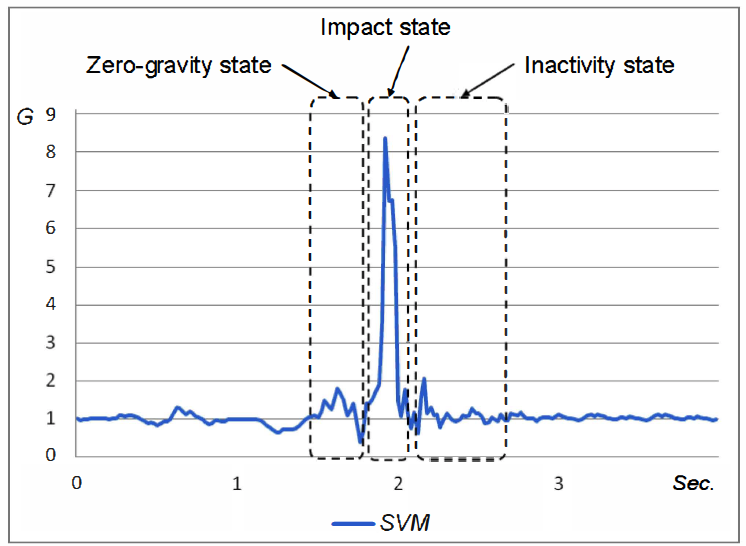
\includegraphics[width=.8\textwidth]{imagens/fall_states.png}
	\caption{Etapas de uma queda \citep{hsieh2014wrist}.}
	\label{fig:fall_states}
\end{figure} 


\begin{itemize}
	\item{\textbf{Período Anterior a Queda (Pre-Fall)}: Durante este período o individuo estará realizando suas atividades cotidianas, que podem levar ou não a um pico de aceleração que deve ser tratado para que se possa evitar falso-positivos. Ações que geralmente levam a este pico de aceleração são movimentos como sentar ou se deitar muito rápido, ou dependendo da posicionamento dos sensores, atividades físicas que exigem bastante movimentação. }
	
	\item{\textbf{Período Anterior a Queda (Pre-Fall)}: Durante este período o individuo estará realizando suas atividades cotidianas, que podem levar ou não a um pico de aceleração que deve ser tratado para que se possa evitar falso-positivos. }
	
	\item{\textbf{Período Queda Livre (Free-Fall)}: Durante este período o individuo está se descolando em direção ao chão. Nesta fase o valor de sua aceleração irá tender a 0.  }
	
	\item{\textbf{Período do Impacto (Impact-Phase)}: Período caracterizado pelo impacto do índividuo, este período é crítico na aplicação, poís é onde ocorre o pico de aceleração. }
	
	\item{\textbf{Período de Inatividade (Inactive State)}: Período posterior a queda, onde o usuário irá realizar o esforço para se levantar. Em quedas mais graves, onde o usuário está incapaz de se movimentar ou inconsciente este valor se modificação de maneira muito sutil, porém de forma geral, o usuário que sofreu uma queda não se levanta imediatamente. De acordo com \cite{mehner2013location}, o período de pós impacto e inatividade levá aproximadamente 2 segundos.  }
	
\end{itemize}


\section{Tipos de Sistemas de Detecção de Queda}
\label{sec:fall_system_types}
Diversos tipos de Sistemas de Detecção de Queda foram desenvolvidos nos últimos anos e estes utilizam diferentes abordagens buscando atingir o mesmo objetivo: realizar a detecção automática das quedas. De acordo com \cite{mubashir2013survey}, estes sistemas podem ser categorizados em três grupos: sistemas de detecção baseados no ambiente, sistemas de detecção baseados na visão, sistemas de detecção baseados em tecnologias vestíveis.

\subsection{Sistemas de Detecção Baseados no Ambiente}
Sistemas de detecção baseados no Ambiente utilizam a fusão de dados obtidos de diversos sensores para realizar a detecção de quedas. Atravês desses sensores são obtidos sinais audio-visuais e dados vibracionais do ambiente que está sendo monitorado. Este tipo de sistema podem ser divididos em duas categorias:

\begin{itemize}
	\item{\textbf{Audio-Visuais}: Neste tipo de sistema são analisados os sinais audio-visuais obtidos atravês de câmeras e microfones espalhados no ambiente desejado. Um exemplo deste sistema foi proposto por \cite{zhuang2009acoustic}, ele utiliza o padrão da onda sonora capturada, com uma base de dados treinada  com diferentes tipos de onda sonoras associadas com diferentes tipos de eventos. Sendo assim, capaz de diferenciar uma queda de uma atividade diária. }
	
	\item{\textbf{Dados Vibracionais}: Neste tipo de sistema são analisados os dados vibracionais obtidos atravês de sensores de vibração espalhados no chão do ambiente desejado. Um exemplo deste sistema foi proposto por \cite{zhuang2009acoustic}, ele utiliza o padrão da onda sonora capturada, com uma base de dados treinada  com diferentes tipos de onda sonoras associadas com diferentes tipos de eventos. Sendo assim, capaz de diferenciar uma queda de uma atividade diária. }
\end{itemize}



\subsection{Sistemas de Detecção Baseados na Visão}
Sistemas de detecção baseados na visão utilizam uma ou mais câmeras posicionadas ao redor do ambiente desejado para  que se possa realizar a detecção de quedas. As camêras são consideradas um meio menos intrusivo de detecção, pois, diferente dos sistemas que utilizam tecnologias vestíveis, somente o video gerado pela câmera são utilizadas na detecção, sem a necessidade do usuário vestir nenhum dispositivo eletrônico. Diferentes tipos de técnicas de processamento de video e imagem são utilizadas na detecção. As principais delas são:  

\begin{itemize}
	\item{\textbf{Espaço-Temporais}: Sistemas que utilizam caracteristicas espaço-temporais para realizar modelagens capazes de fornecer dados cruciais na detecção de diferentes tipos de atividades.  Um sistema proposto por \cite{foroughi2008eigenspace} realiza a extração de informações de movimento de uma sequência de video. Aplicando uma técnica chamada Eigenspace sobre as informações de movimento coletadas, é possível extrair um vetor de caracteristicas, que  é utilizado por um algoritmo de inteligência artificial, mais especificamente um algoritmo de redes neurais, para determinar o tipo de evento ocorrido. }
	
	\item{\textbf{Inatividade/Mudança de Forma}: Sistemas que utilizam mudanças de forma e ausência de atividade no monitoramento em video para realizar a detecção de quedas. Um exemplo deste tipo de sistema foi proposto por \cite{rougier2011robust}. Em seu artigo, são utilizadas técnicas de detecção e análise de formas para detectar a silhueta e atividade (representado por mudanças de forma) do indíviduo que está sendo monitorado. Para que se possa diferenciar quedas das atividades diárias, é utilizado o método de \textit{Mistura de Modelos Gaussianos}, um método estastístico utilizado em visão computacional.}
	
	\item{\textbf{Postura}: Sistemas que identificam e localizam diversas posturas do individuo, calculadas através das diferentes posições corporais, utilizando uma sequência de imagens para realizar a detecção um evento de queda. \cite{cucchiara2005probabilistic}, desenvolveu um sistema de detecção que analisa os histogramas das imagens geradas pelas câmeras, para classificar as posturas do individuo monitorado e consequentemente detectar um evento de queda.  }
	
	\item{\textbf{Análise 3D da Posição da Cabeça}: Sistemas que realizam o monitoramento da cabeça do individuo, e atravês de modelos de estado é capaz de detectar as magnitudes do movimento realizado. Um exemplo deste tipo de sistema foi proposto por \cite{rougier2005demo}, ele realiza a modelagem 3D da cabeça do individuo e capaz de calcular a velocidade e a trajetória deste modelo que são posteriormente utilizadas na categorização do evento como queda.}	
\end{itemize}



\subsection{Sistemas de Detecção Baseados em Tecnologias Vestíveis}
Sistemas vestíveis de detecção de quedas utilizam os dados de sensores que estão acoplados sobre ou na roupa dos usuários. Este tipo de sistema apresentam claras vantagens sobre tanto os sistemas baseados no ambiente ou na visão. Ambos os tipos de sistema, exigem um custo constante de manuntenção, que dependendo de como o sistema foi desenvolvido, pode ser bastante alto, além disso a área de atuação do sistema fica limitada a uma área pré-determinada (e.g quarto, sala de estar). Utilizando tecnologias véstiveis não temos este problema, pois o usuário poderá leva o seu dispositivo para onde ele desejar.

Levando em consideração a privacidade do usuário, os sistemas vestíveis levam vantagem em relação aos baseados no ambiente e na visão. A necessidade de uma monitoração por vídeo constante necessária em alguns desses sistemas podem deixar o usuário relutante em implementar está solução. 

De acordo com \cite{igual2013challenges}, o uso de smartphones para realizar a detecção de quedas tem sido uma tendência devido ao seu baixo preço, altos volumes de produção e facilidade de desenvolvimento. O grande problema do uso do smartphone é justamente o seu posicionamento. O aparelho pode estar em diversas posições, ou mesmo, nem diretamente ligado ao corpo do usuário. Está incerteza dificulta bastante o uso deste tipo de dispositivo no reconhecimento de atividades. 

Tentando resolver este problema, o uso de aparelhos realmente vestíveis vem sendo utilizado em sistemas de detecção de quedas, como pode ser visto nos trabalhos desenvolvidos por \cite{hsieh2014wrist} e \cite{pivato2011wearable}.



\chapter{Sistemas Vestíveis} 
\label{cap:wearablw_systems}

Sistemas Vestíveis podem ser definidos como dispositivos eletrônicos móveis que podem ser discretamente embutidos nos trajes do usuário, como parte da roupa ou um acessório. Diferente dos sistemas móveis convencionais, eles podem funcionar sem ou com muito pouca interferência nas atividades do usuário \citep{lukowicz2004wearable}. 

Hoje, muitos destes dispositivos vestíveis vem com uma gama de sensores embutidos que são utilizados na detecção de quedas. O tipo de sensor mais comum utilizado em \ac{FDS} é o acelerômetro, com alguns desses sistemas também utilizando o giroscópio como um sensor auxiliar. De acordo com a revisão sistemática feito por \cite{igual2013challenges}, 186 dos 197 sistemas analisados utilizam o acelerômetro como sensor principal na detecção de quedas. A utilização desde sensores em \ac{FDS} se deve muito pela popularização e o barateamento dos mesmos, além da utilização desses sensores embarcados em smartphones e smartwatches.


As seções desse capítulo são organizadas da seguinte maneira: A seção \ref{sec:sensors} descreve os principais tipos de sensores utilizados em \ac{FDS}; A \ref{sec:sensor_position} fala sobre o posicionamento de sensores, fazendo uma correlação entre o posiciomanento dos sensores e a accurâcia dos sistemas estudados; A seção \ref{sec: FDS_algorithm} fala sobre os diferentes tipos de algoritmos de detecção de quedas mostrando suas vantagens e desvantagens; Por fim, a seção \ref{sec:FDS_examples} irá mostrar exemplos de aplicações que realizam a detecção de quedas atravês de tecnologias vestíveis. 



\section{Sensores}
\label{sec:sensors}
A escolha e o bom funcionamento de sensores são uma parte essencial no bom funcionamento de sistemas de detecção de quedas. De forma geral, sensores são dispositivos que convertem fenômenos físicos em sinais elétricos. Sendo assim , eles representam a camada de comunicação entre o mundo físico e o mundo digital. 

Os dois tipo principais de sensores utilizados em sistemas de detecção de queda são o acelerômetro e o giroscópio. Eles fazem parte de um grupo chamado de \ac{MEMS}. Estes sensores são geralmente feitos de chips de silício utilizando as mesmas técnicas usadas na confecção de chips de computadores pessoais. Para que um sensor possa ser classificado como \ac{MEMS} alguma parte do seu design precisa vibrar ou se mover de alguma forma \citep{milette2012professional}. 

De forma geral tanto o acelerômetro quanto o giróscopio utilizam 3 eixos para expressar seus valores. O sistema de coordenadas utilizado é relativo a cada dispositivo. Na figura \ref{fig:axis_device} temos  exemplo do sistemas de coordenadas utilizado pelo sistema operacional Android\footnote{https://www.android.com/}. Neste sistema o ponto de origem é o centro da tela do dispositivo, quando segurado na posição vertical \citep{sensorAndroidDocs}. 

\begin{figure}[ht]
	\centering
	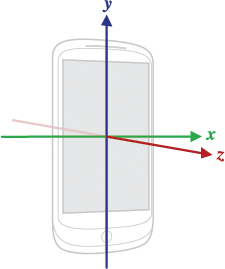
\includegraphics[scale=0.6]{imagens/axis_device.png}
	\caption{Sistema de coordenadas utilizado pelo sistema operacional Android \citep{sensorAndroidDocs}.}
	\label{fig:axis_device}
\end{figure} 

\subsection{Acelerômetro}
\label{subsec:accelerometer}
Fisicamente, o acelerômetro é um dispositivo composto de uma pequena massa  anexado a pequenas molas que são utilizadas para medir a aceleração aplicada sobre um dispositivo, incluindo a força da gravidade. A aceleração é medida analisando o quanto a massa se distancia do seu ponto de equilíbrio. 

\begin{figure}[ht]
	\centering
	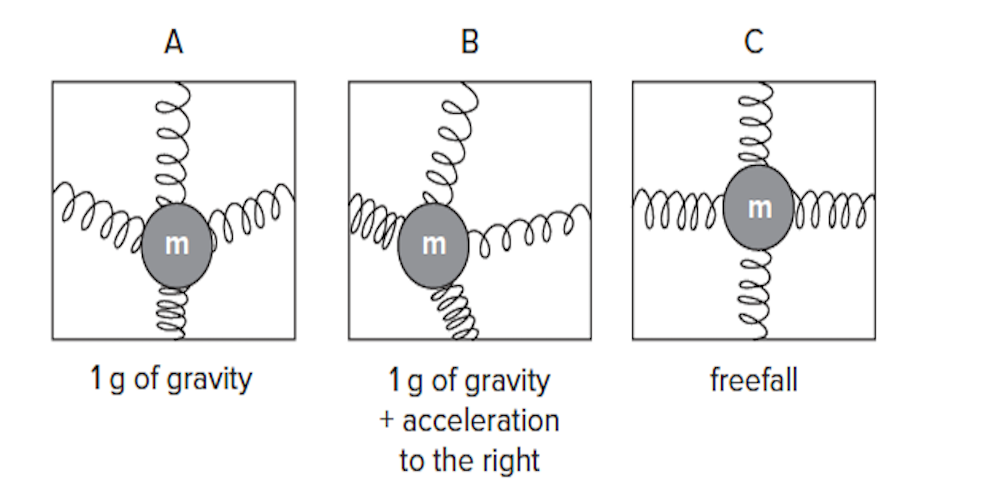
\includegraphics[scale=0.6]{imagens/MEMS_device.jpg}
	\caption{Força sendo aplicando sobre uma massa presa a molas \citep{milette2012professional}.}
	\label{fig:acelerometro}
\end{figure} 

	
Na figura \ref{fig:acelerometro} em A é possível ver um aparelho parado em uma mesa, sobre ele só irá agir a força de gravidade 1G de aproximadamente $9.8 m/s^{2}$. Em  B, o aparelho foi jogado para a direita, então irá agir sobre ele, além da força da gravidade, uma aceleração no sentido para onde o aparelho se movimentou. Já em C, vemos um aparelho em queda livre com aceleração no sentido oposto a força da gravidade, o que faz com a massa fique localizada em seu ponto de equilibrio, e a força resultante  seja de $0G$ \citep{milette2012professional}.


\subsection{Giroscópio}
	
	O giroscópio, similarmente aos acelerômetros, são pequenas massas em pequenas molas, só que em vez de medir a aceleração, são utilizados para medir um tipo de força chamada de Força de Coriolis. A Força de Coriolis é a tendência que um objeto livre possui de sair do curso quando visto de um ponto de referência em rotação \citep{milette2012professional}. Por exemplo, se sentarmos em um carrosel e rolarmos a bola pra longe, a bola irá parece desviar em uma linha reta, como se existisse uma força agindo sobre ela. Esta força é chamada de Força de Coriolis.
	
	Apesar de possuir uma estrutura física semelhante, o aceletrometro e o giroscópio se diferem em seu funcionamento. Em vez de esperar a força da gravidade agir sobre a massa, o giroscópio funciona vibrando está massa sobre o eixo definido. Quando o giroscópio é rotacionado, a Força de Coriolis faz com que a massa comece a ser mover em um eixo dirente no qual ele estava vibrando anteriomente.  \cite{milette2012professional}.
	
	Como a força de Coriolis age somente quando o dispositivo está em rotação, o giroscópio só é capaz de calcular a velocidade angular, ou seja, a velocidade com que o aparelho está sendo rotacionado. 
	
	A orientação da dispositivo irá definir quando o valor da rotação será positivo ou negativo. Nos dispositivos Android, a velocidade Angular é medida em radianos por segundo ($rad/s$) e é positiva em rotações no sentido anti-horário \citep{GyroscopeAndroidDocs}. 
	
\section{Posicionamento de Sensores}
\label{sec:sensor_position}

O posicionamento dos sensores afeta diretamente a performance dos \ac{FDS}, dependendo da posição onde colocamos os sensores, o sistema pode indicar uma maior ou menor quantidade de falhas. 

Não existe um consenso sobre a posição otimizada dos sensores para que se possa realizar a detecção de quedas. De acordo com \cite{abbate2011recognition}, a cintura seria o local ideal para o posicionamento, já que estaria mais perto do centro de gravidade do corpo humano. Entretanto em \cite{kangas2007determination}, já foi sugerido que a cabeça seria o melhor lugar para posicionar os sensores. Outras soluções, como em \cite{gjoreski2011accelerometer}, já propõem o uso de mais de um sensor, colocando-os em diferentes partes do corpo com o objetivo de aumentar ainda mais a precisão dos \ac{FDS}.


De acordo com X, o pulso não é o local recomendado para o posicionamento de sensores em sistemas de detecção de quedas. Isso se deve  a constante movimentação dos braços, que podem gerar um número grande de falso-positivos. Entretanto, alguns sistemas tem conseguido resultados satisfatórios com \ac{FDS} localizados no pulso. O sistema proposto por \cite{hsieh2014wrist}, foi capaz detectar quedas em 151 das 160 quedas simuladas e obteve uma especificidade (capacidade de não reconhecer eventos de quedas, como tal) de 95\%.

Além da acurrácia do sistema, outras questões precisam ser levadas em consideração quando pensamos no posicionamento dos sensores. Uma delas é a danificação dos sensores na occorrência de uma queda. Caso o sistema pare de funcionar, um possível alerta de emergência poderá não ser enviado e o idoso poderá está correndo grande perigo. 

Outra questão é a usabilidade, o uso de muitos sensores, apesar de poder elevar a precisão do sistema, poderá levar a um disconforto do usuário, que pode fazer até com que o mesmo desista de usá-lo. 


\section{Algoritmos de Detecção de Queda}
\label{sec: FDS_algorithm}
Os algoritmos de detecção de quedas recebem como entrada os dados obtidos através dos sensores e são capazes de determinar se o que ocorreu foi um evento de queda ou somente uma \ac{ADL}. De acordo com \cite{casilari2015analysis}, é possível separar os algoritmos de detecção em dois grandes grupos: Algoritmos de detecção através de métodos de reconhecimento de padrões, algoritmos baseados em limiares. 




\subsection{Reconhecimento de Padrões}
O reconhecimento de padrões é uma área do aprendizado de máquina que foca no reconhecimento de padrões e regularidades de dados \citep{anzai2012pattern}. Diversas técnicas de aprendizado de máquina tem sido empregadas na detecção de quedas, de acordo com a revisão sistemática feita por \cite{casilari2015analysis}, algoritmos como o de \textit{Naïve Bayes}, \textit{Redes Neurais}, e \textit{Árvores de Decisão} tem sido utilizados.


Um exemplo de sistema que utiliza a técnica de reconhecimento de padrões foi proposto por \cite{zhao2012fallalarm}. O seu algoritmo de detecção de quedas analisa dados do acelerômetro através de uma árvore de decisão, assim identificando um evento de queda. 

Este algoritmo é composto de 2 fases, a primeira é o que chamamos em aprendizado de máquina de fase de treinamento. Será realizado a coleta de dado e a  extração das características que são pertinentes, além do treinamento de um modelo de árvore de decisão. Na figura \ref{fig:decision_tree} podemos ver o modelo de árvore de decisão gerado.  Este modelo de árvore de decisão é capaz de reconhecer atividades como andar, correr, estado estático ou um evento de queda através das variáveis \textit{Std\_x}, \textit{Mean\_y} e \textit{Slope} que representam caracteristicas do sistema. 


\begin{figure}[ht]
	\centering
	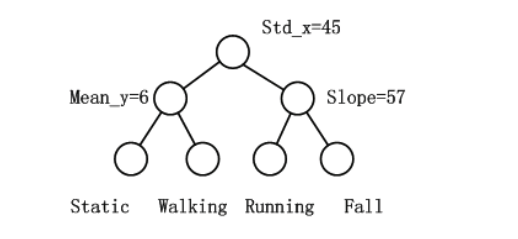
\includegraphics[scale=0.6]{imagens/decision_tree.png}
	\caption{ Modelo de árvore de decisão construida em \cite{zhao2012fallalarm}.}
	\label{fig:decision_tree}
\end{figure} 


Na segunda fase, chamada de fase de testes, o modelo de árvore de decisão é utilizado em uma aplicação no smartphone que será responsável pelo reconhecimento de atividades. Os dados dos sensores são catalogados e transformados nas caracteristicas do sistema, que serviram como dados de entrada da árvore de decisão, que terá como saída o tipo de atividade que foi desempenhada.

Sistemas que utilizam reconhecimento de padrões, normalmente está suscetível a altos custos computacionais, análise massiva de dados, e acesso a grandes bancos de dados ou longos periodos de treinamentos onde o algoritmo de classificação precisa ser parametrizado e adaptado a diferentes grupos de usuários \citep{casilari2015analysis}. Em constraste, existem os algoritmos baseados em limiares que tendem a ser mais simples e similarmente eficientes, desde que encontremos limiares adequados. 

\subsection{Baseado em Limiares}
Algoritmos baseados em limiares utilizados na detecção de quedas comparam os dados dos sensores com um ou mais valores pré-definidos, chamados de limiares. Estes valores podem ser fixos ou adaptados. Quando estes valores são adaptados, eles não mudam dinamicamente enquanto os usuários estão utilizando o sistema. Em vez disso, o usuário irá introduzir dadados sobre o seu perfil fisiológico e o sistema irá informar os limiares adequados \citep{habib2014smartphone}. Um exemplo deste tipo de sistema pode ser visto em \cite{sposaro2009ifall}, o valor limiar mudar de acordo com os parametros providos pelo usuário como altura, peso e nível de atividade. 

De acordo com a revisão sistemática feito por \cite{casilari2015analysis}, muitos sistemas de detecção de queda utilizam o valor de \ac{SMV} do vetor de aceleração como  valor limiar principal em seus algoritmos de detecção. O valor de \ac{SMV} é definido através da equação em \ref{eq:SMV}, onde $X_i$, $Y_i$, $Z_i$, representam, respectivamente, os valores de aceleração dos eixos x, y, z obtidos através do acelerômetro descrito em  \ref{subsec:accelerometer}.

\begin{equation}
SMV = \sqrt{X_i^2 + Y_i^2 + Zi_i^2} 
\label{eq:SMV}
\end{equation}

A escolha dos limiares é um fato determinante para o sucesso deste tipo de algoritmo de detecção de quedas. A escolha dos limiares pode ser feita atravês de experimentos preliminares como em \cite{zhang2013honey}. Em seu trabalho, um grupo de voluntários foi escolhido para realizar diversas \ac{ADL}, como andar, correr subir e descer escadas e também realizar a simulação de quedas. Através dos dados obtidos foi possível descobrir os limiares de \ac{SMV} para um evento de queda.  

De acordo com \cite{cao2012falld}, a performance dos algoritmos aumenta significadamente quando utilizamos valores de limiar dinâmicos. De acordo com sua pesquisa, o número de eventos de queda que não foram caracterizadas como tal, cairam de 53 para 29 quando o peso, sexo idade foram levados em consideração no momento da definição dos limiares.

Outra questão importante quando utilizado este tipo de algoritmo é o número de limiares utilizados. De acordo com \cite{casilari2015analysis}, o uso de um único limiar faz com que o algoritmo emita um número grande de alerta falsos, categorizando \ac{ADL} como eventos de queda, fazendo com que o uso de somente um limiar não seja adequado no desenvolvimento de \ac{FDS}.


\section{Trabalhos Relacionados}
\label{sec:FDS_examples}
Como vimos no decorrer desse trabalho, não existe na literatura um algoritmo ou dispositivo padrão para o desenvolvimento de \ac{FDS}. A plataforma vestível é bastante promissora por estar naturalmente aclopada a alguma parte do corpo do usuário, sendo possivel criar um algoritmo de detecção mais confiáveis, já que, como visto em \cite{casilari2015analysis}, grande parte dos algoritmos de detecção de quedas tem como pré-condição para o seu bom funcionamento, que o dispositivo esteja localizado em uma posição fixa do corpo, como cintura, pulso ou cabeça. Sendo assim, falaremos sobre três sistemas de detecção de quedas que embarcaram os seus sistemas de detecção de quedas em plataformas vestíveis. 

\subsection{SPEEDY - Detector de Quedas em um Relógio de Pulso}
SPEEDY foi o primeiro protótipo de um relógio detector de quedas construido em um smartwatch \citep{degen2003speedy}. Em seu trabalho, ele só utilizou um 2 sensores que são capazes de medir a aceleração através de 3 eixos \textit{x, y, z}. Na figura \ref{fig:speedy} é possível ver o protótipo do sistema desenvolvido e os 3 eixos utilizados para calcular o valor da aceleração. 

\begin{figure}[ht]
	\centering
	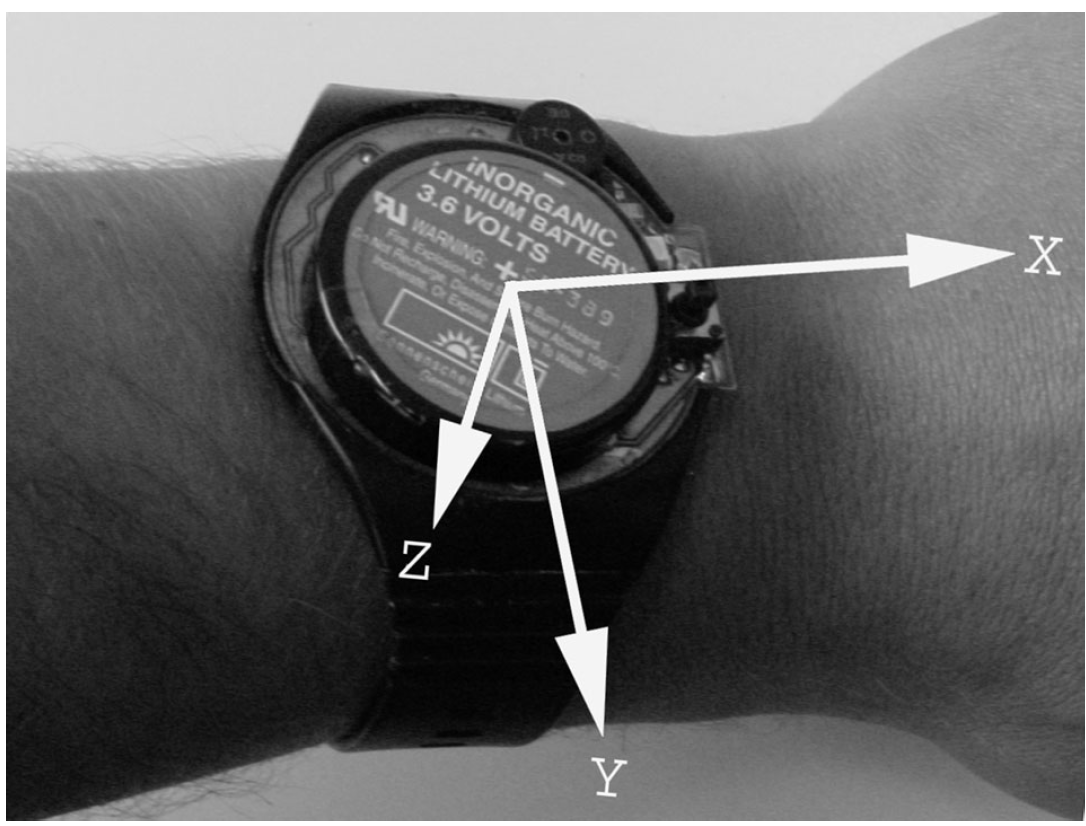
\includegraphics[scale=0.5]{imagens/speedy.png}
	\caption{ SPEEDY e seus eixos \cite{degen2003speedy}.}
	\label{fig:speedy}
\end{figure} 

O algoritmo de detecção de quedas do Speedy utiliza um algoritmo baseado em limiares com 3 valores distintos: o valor de \ac{SMV} calculado através da formula que pode ser vista em \ref{eq:SMV}, dois valores de velocidade distintos chamados de $v_1$ e $v_2$. A velocidade $v_1$ é o valor aproximado da velocidade vertical (de queda), e o valor da velocidade $v_2$ representa a velocidade do dispositivo Speedy. 

No primeiro passo do algoritmo, um alto valor de velocidade precisa ser identificado indicando uma possível queda. Depois disso, nos próximos 3 segundos um impacto precisa ser detectado, representado por alto valores de aceleração. Depois disso, o usuário é observado por mais 60 segundos, se durante este tempo, pelo menos 40 segundos forem marcados por inatividade um alerta sonoro é emitido. 

O Speedy foi avaliado através de quedas simuladas por 3 individuos diferentes em um colchão. Cada indivíduo simulou  quedas em 3 posições diferentes: Frente, lado, costas. Foram realizadas um total de 45 quedas, onde 65\% delas foram corretamente marcadas como um evento de queda. 

\subsection{F2D - Sistema de Detecção de Quedas}
\label{subsec:F2D_System}
F2D é uma applicação Android embarcado em um smartwatch \textit{AW-420.RX} da Simvalley Mobile\footnote{http://www.simvalley-mobile.de/} \citep{kostopoulos2015f2d}. O algoritmo implementado no F2D tem como entrada os dados do acelerômetro, levando em consideração os movimentos realizados depois de um evento de queda e a localização do usuário. 

Para que se possa detectar as quedas, o F2D utiliza um algoritmo baseado em limiares, onde os limiares foram definidos utilizando um banco de dados com mais de 150 eventos simulados de queda. O algoritmo de detecção de quedas presente no F2D é composto de quatro etapas\citep{kostopoulos2015f2d}:

\begin{enumerate}
	
	\item{\textbf{Padrão de Queda}: Para que um evento possa ser identificado como uma possível queda, o valor da aceleração precisa ultrapassar um limite que varia de $10 m/s^{2}$ a $18 m/s^{2}$ que representa o impacto da queda, e depois de um intervalo de tempo, precisa ultrapassar um limiar de $2 m/s^{2}$  a $7 m/s^{2}$, caracterizado como o movimento residual da queda. Tanto os valores exatos dos limiares, quanto o intervalo de tempo entre a análise dos mesmos variam de acordo com perfil do usuário.   }
	
	\item{\textbf{Módulo de Decisão}: Toda vez que ambas as condições da etapa anterior são satisfeitas é acrescido 1 em um contador. São estabelecidos dois valores $X$ e $Y$. O valor de $X$ representa o limiar do contador e $Y$ representa o seu limite. Sendo assim, o valor do contador precisa ficar entre X e Y, ou seja, $ X \leq Contador < Y $. Caso este valor seja maior que Y, outra atividade estava sendo desempenhada, como por exemplo correr, e caso este valor do contador seja menor que X, onde $X = 1$, então um movimento brusco do braço aconteceu, mas que não caracteriza uma queda.  }
	
	\item{\textbf{Ação posterior a Queda}: Logo depois que um evento é caracterizado como queda, o F2D é capaz de identificar se o usuário conseguiu se recuperar, e volto a exercer suas atividades normais, caso isto ocorra, o sistema não irá emitir um alerta para o seu cuidador, caso contrário, um alerta é emitido }
	
	\item{\textbf{Ação baseada na Localização}: O F2D também se baseia na localização do usuário. Caso este esteja na rua, e todas as etapas anteriores se concretizaram, um alarme é enviado para o cuidador. Caso o usuário esteja em casa, o sistema faz uso da tecnologia \textit{iBeacon} para categorizar certos locais como seguros ou potencialmente perigosos. O iBeacon utiliza o sistema de detecção de proximidade do \ac{BLE} para enviar um identificador único para aplicações ou sistemas operacionais compatíveis que estejam ao alcance do mesmo \citep{kostopoulos2015f2d}.  Caso o local esteja marcado como potencialmente perigoso, uma mensagem é enviada ao cuidador, caso contrário, o usuário terá a oportunidade de cancelar o envio, em um possível evento de queda.}     
	
	
\end{enumerate}


\subsection{Sistema de Detecção de Quedas de Pulso}
O sistema proposto por \cite{hsieh2014wrist} utiliza dois dispositivos vestíveis acoplados no pulso do usuário como pode ser visto na figura \ref{fig:wrist_worn}. 


\begin{figure}[ht]
	\centering
	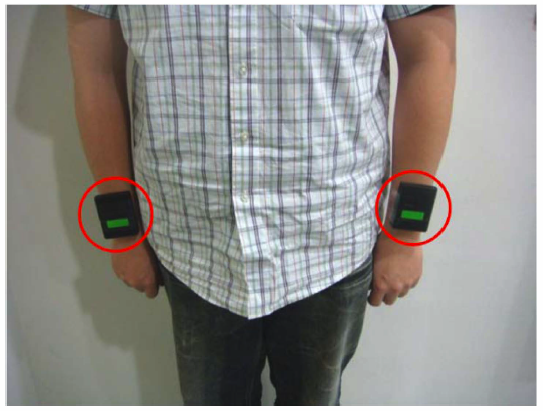
\includegraphics[scale=0.4]{imagens/wrist_worn.png}
	\caption{ Dispositivos véstiveis marcados em vermelho. \cite{hsieh2014wrist}.}
	\label{fig:wrist_worn}
\end{figure} 


Cada um dos dispositivos está equipado com um módulo Zigbee\footnote{http://www.zigbee.org/} responsável pela transmissão dos dados e  um acelerômetro e  giroscópio de 3 eixos. A frequência tanto do acelerômetro quanto do giroscópio foram configuradas para $50 Hz$, ou seja, os dados são coletados a cada \textit{20 ms}.


O algoritmo proposto utiliza ambos os dados do acelerômetro e do giroscópio para realizar a detecção de quedas. Os dados do giróscopio funcionam como um filtro inicial, desconsiderando a maioria das ativididades cotidianas, enquanto os dados do acelerômetro são responsáveis por realizar o julgamento final. O algoritmo utilizado, assim como os demais, é baseado em limiares onde os limiares foram definidos atravês de um treinamento inicial. 

O algoritmo proposto é capaz de diferenciar \ac{ADL} como bater palmas e deitar-se, de um evento de queda em 95\% dos casos. A principal desvantagem do sistema proposto é a necessidade de se utilizar 2 dispositivos, podendo torna-se desconfortável para o usuário.








%\chapter{Modelo de Usuário} 
\label{cap:userModel}

O conjunto finito de propriedades e características do candidato a receber recomendações é o modelo do usuário. O modelo de usuário representa o usuário, ou seja, codifica suas preferências e necessidades \citep{ricci2011recommender}. Várias abordagens para modelagem de usuário têm sido utilizadas e, de certo modo, um sistema de recomendação pode ser visto como uma ferramenta que gera recomendações construindo e explorando modelos de usuário \citep{Berkovsky:2009:CMU:1499116.1499121}. Desde que não é possível fazer recomendações sem um modelo de usuário, a não ser que a recomendação não seja personalizada, o modelo de usuário sempre terá um papel central.

A informação que constitui o modelo de usuário pode variar de acordo com o domínio do sistema de recomendação. Por exemplo, no caso de um sistema de recomendação de filmes, o modelo será constituído pelos filmes que ele gosta de assistir, filmes que não gosta, os atores dos filmes que assiste, gênero etc.


\section{Feedback do Usuário}

Seja qual for a tecnologia específica explorada pelo sistema de recomendação, ela pode fornecer recomendações de alta qualidade apenas depois de ter modelado suas preferências \citep{Berkovsky:2008:MUM:1380736.1380749}. A tarefa de coletar dados de modelagem de usuário é normalmente realizada de duas maneiras:

\begin{itemize}
	\item{\textbf{Explícita}: Através do fornecimento das informações solicitadas explicitamente pelo usuário.}
	
	\item{\textbf{Implícita}: Através da aplicação de vários mecanismos de raciocínio que infere as informações necessárias com base no comportamento observável do usuário \citep{Hanani:2001:IFO:598287.598363}.}
\end{itemize}

A coleta explícita de dados de modelagem do usuário é considerada uma tarefa  precisa, mas que consome tempo e esforço, e por isso é normalmente evitada pelo usuário. Alternativamente, a coleta implícita envolve mecanismos de raciocínio automatizados, os quais podem interpretar errado o comportamento do usuário \citep{Berkovsky:2008:MUM:1380736.1380749}. Na prática, as abordagens explícitas e implícitas podem também ser combinadas.

De modo geral, a qualidade das recomendações fornecidas pelo usuário depende muito das características do modelo de usuário, por exemplo, quão preciso ele é, qual a quantidade de informação que ele armazena, e se essa informação está atualizada. Assim, como uma regra geral, quanto mais informação é armazenada no Modelo de Usuário, isto é, quanto mais conhecimento tem obtido sobre o usuário, melhor será a qualidade da recomendação. Neste contexto, qualidade refere-se à capacidade do sistema de sugerir exatamente aqueles produtos ou serviços que o usuário irá selecionar e comprar, ou predizer corretamente aqueles itens que o usuário irá gostar \citep{Berkovsky:2008:MUM:1380736.1380749}. Na prática, obter dados de modelagem de usuário suficientes para entregar recomendações de alta qualidade é difícil. Isso é especialmente importante nos estágios iniciais de interação com o usuário, quando pouca informação sobre o usuário está disponível. Nestes estágios, todas as técnicas de recomendação enfrentam o problema da "partida a frio", isto é, a situação onde a informação disponível sobre o usuário e/ou itens não é suficiente para fornecer recomendações de alta qualidade \citep{Linden:2003:ARI:642462.642471}.


\section{Modelagem}

Cada sistema de recomendação constrói e mantém uma coleção proprietária de Modelos de Usuário \citep{Montaner:2003:TRA:640471.640491}. Praticamente, isto significa que os dados de modelagem de usuário coletados são adaptados para:

\begin{itemize}
	\item{o conteúdo específico (produtos ou categoria de produtos) oferecido pelo sistema de recomendação, por exemplo, filmes, músicas, notícias, etc.}
	
	\item{a técnica de recomendação sendo explorada pelo sistema, por exemplo, filtragem colaborativa, filtragem baseada em conteúdo, ou alguma híbrida.}
\end{itemize}

Assim, uma enorme quantidade de dados heterogêneos de modelagem de usuário são disseminados entre vários sistemas. Entretanto, sistemas de recomendações na prática (especialmente os comerciais) não permitem outro sistema de recomendação externo acessá-los, como também não compartilha seus dados de modelagem de usuário. Apesar disso, é razoável supor que sistemas de recomendação podem potencialmente beneficiar-se de enriquecer seus dados de modelagem de usuário importando e integrando dados de modelagem de usuário coletados por outros sistemas de recomendação, e portanto fornecer melhores recomendações para o usuário \citep{Berkovsky:2008:MUM:1380736.1380749}.

\cite{Kobsa1994}, para evitar caracterizar modelagem de usuário através de estruturas e processos, listou os seguintes serviços frequentemente encontrados nos sistemas de modelagem de usuário:

\begin{itemize}
	\item{a representação de suposições sobre um ou mais tipos de características de usuário em modelo de usuários individuais (por exemplo, suposições sobre seu conhecimento, equívocos, objetivos, planos, preferências, tarefas, e habilidades);}
	
	\item{a representação de características relevantes comuns de usuários que pertencem a um específico subgrupo do sistema (o chamado, estereótipo);}
	
	\item{a classificação dos usuários como pertencentes a um ou mais destes subgrupos, e a integração das características típicas destes subgrupos dentro do modelo de usuário individual atual;}
	
	\item{o registro do comportamento dos usuários, particularmente sua interação passada com o sistema;}
	
	\item{a formação de suposições sobre o usuário baseado no histórico de interações;}
	
	\item{a generalização do histórico de interações de muitos usuários em estereótipos;}
	
	\item{o desenho de suposições adicionais sobre o usuário atual baseado em valores iniciais.}
	
	\item{manutenção de consistência no modelo de usuário;}
	
	\item{o fornecimento da suposição atual sobre o usuário, como também justificativas para estas suposições;}
	
	\item{a avaliação das entradas no modelo de usuário atual, e a comparação com padrões.}
\end{itemize}

Segundo \cite{Kobsa:2001:GUM:598284.598347}, os seguintes requisitos para os sistemas de modelagem de usuário são considerados importantes:

\begin{itemize}
	\item{\textbf{Generalidade, incluindo independência de domínio}: Os sistemas precisam ser utilizáveis por quantas aplicações e domínios de conteúdo for possível, e dentro destes domínios por quantas tarefas de modelagem de usuário for possível.}
	
	\item{\textbf{Expressividade}: Os sistemas precisam expressar quantos tipos de suposições sobre o usuário forem possíveis ao mesmo tempo.}
	
	\item{\textbf{Capacidade Inferencial Forte}: Os sistemas precisam realizar todo tipo de raciocínio que são tradicionalmente distinguidos em inteligência artificial e lógica formal.}
\end{itemize}






\section{Modelos de Usuário Baseados em Múltiplos Domínios}

Sistemas de recomendação é um campo de pesquisa ativo e vem sendo utilizado com sucesso em um grande número de sistemas como Netflix\footnote{http://www.netflix.com}, Youtube\footnote{http://www.youtube.com}, iTunes\footnote{http://www.apple.com/itunes/}. A grande maioria destes sistemas oferecem recomendações apenas para itens pertencentes a um único domínio. Nestes casos, as recomendações são computadas utilizando feedback do usuário (avaliação) sobre itens no domínio alvo. Em sites de \textit{e-commerce}, como Amazon\footnote{http://www.amazon.com}, no entanto, seria útil explorar avaliações do usuário sobre diversos tipos de itens para gerar um modelo mais geral das preferências do usuário. De fato, pode existir dependências e correlações entre as preferências entre diferentes domínios e ao invés de tratar cada tipo (por exemplo, eletrônicos e música) independentemente, o conhecimento do usuário adquirido em um domínio pode ser transferido e explorado em muitos outros domínios \citep{fernandez2012cross}.

Além disso, um sistema pode oferecer recomendações personalizadas de itens em múltiplos domínios, por exemplo, sugerir não apenas um filme em particular, mas também CDs de música, livros ou videogames que de alguma maneira estejam relacionados com o filme. Analogamente, em uma aplicação turística seria de grande valor sugerir um evento cultural para cliente que tenha reservado um quarto em um hotel recomendado, ou em sistema de e-learning, apresentar um estudante com referências bibliográficas relacionadas a uma vídeo-aula que tenha sido recentemente recomendada \citep{fernandez2012cross}.

Um dos primeiros estudos relacionados a recomendações em múltiplos domínios foi apresentado por \citep{Winoto2008}. Eles identificaram três importantes questões a serem investigadas:

\begin{itemize}
	\item{Verificar a existência de correlações globais das preferências do usuário para itens em diferentes domínios.}
	
	\item{Criar modelos capazes de explorar as preferências de usuário em um domínio fonte para predizer as preferências de usuário em domínio alvo}
	
	\item{Desenvolver avaliações apropriadas para recomendações em múltiplos domínios.}
\end{itemize}

\cite{Winoto2008} acreditavam que, embora recomendações entre múltiplos domínios tendessem a ser menos precisas do que recomendações em um único domínio, a primeira seria mais diversificada, o que pode levar a uma maior satisfação do usuário \citep{Adomavicius:2005:TNG:1070611.1070751}. Além disso, recomendações entre múltiplos domínios tem outras vantagens, como lidar com o problema da partida-a-frio (cold-start problem) \citep{Abel2012}, e também o problema da esparsidade \citep{Li:2009:MBC:1661445.1661773}, \citep{AAAI101649}. Ao identificar as relações entre itens em dois domínios diferentes, pode-se sugerir para um usuário com itens em um domínio inexplorado, simplesmente explorando suas preferências para os itens em outros domínios conhecidos.





\section{Ranking Personalizado}
O objetivo de um ranking personalizado é fornecer para um usuário uma lista ordenada de itens. Um exemplo é uma loja online que pretende recomendar uma lista personalizada e ranqueada de itens que o usuário poderia querer comprar. Em sistemas de feedback implícito, apenas observações positivas estão disponíveis.  Os itens não avaliados pelo usuário (por exemplo, um usuário que não tenha comprado um item ainda) são uma mistura de feedback negativo real (o usuário não está interessado em comprar o item) e falta de valores (o usuário pode querer comprar o item no futuro).


\subsection{Bayesian Personalized Ranking}

\ac{BPR} é um framework genérico para otimizar diferentes tipos de modelos baseado em treinar dados contendo apenas feedbacks implícitos. \ac{BPR} é baseado na ideia de reduzir a classificação para pares de classificação \citep{balcan2008}. Foi proposto por \citep{Rendle:2009:BBP:1795114.1795167} para lidar com o problema ao treinar um modelo de recomendação de itens utilizando apenas feedbacks implícitos baseado apenas em dados positivos e negativos. O modelo será levado a fornecer pontuações positivas para os itens observados, enquanto considerará itens não visitados como negativo. Entretanto, tal suposição é imprecisa porque um item não observado pode ser pelo fato de que não é conhecido pelo usuário.

Considerando este problema, ao invés de treinar o modelo utilizando apenas os pares usuário-item, \cite{Rendle:2009:BBP:1795114.1795167} propôs considerar a ordem relativa entre um par de itens, de acordo com as preferências do usuário. Sendo $N(u)$ o conjunto de itens para o qual o usuário $u$ forneceu feedback implícito e $\bar{N}(u)$ o conjunto de itens desconhecidos pelo usuário $u$, é inferido que se um item $i$ foi visto por um usuário $u$ e $j$ não foi visto ($i \in N(u)~$ e $j \in \bar{N}(u)$), então $i >_{u} j$, o que significa que ele prefere $i$ ao invés de $j$.


\subsection{BPR-Linear}
\label{sec:bpr-linear}
O BPR-Linear \citep{gantner2010} é um algoritmo baseado no framework \ac{BPR}, que utiliza atributos de item em um mapeamento linear para estimar pontuação. A regra de predição é definida como:

\begin{equation}
\hat{r}_{ui} = \phi_f(\vec{a}_i) = \displaystyle\sum_{g=1}^{n} w_{ug} a_{ig}~~,
\label{eq:bpr-linear}
\end{equation}

\noindent onde $\phi_f : \mathbb{R}^n \rightarrow \mathbb{R}$ é uma função que mapeia os atributos do item para as preferências gerais $\hat{r}_{ui}$ e $\vec{a}_i$ é um vetor booleano de tamanho $n$ onde cada elemento $a_{ig}$ representa a ocorrência ou não de um atributo, e $w_{ug}$ é uma matriz de peso gerado utilizando LearnBPR, que é uma variação da técnica "stochastic gradient descent" \cite{gantner2011}. Desta maneira, nós primeiro calculamos a importância relativa entre dois itens:

\begin{equation}
\begin{array}{ll}
\hat{s}_{uij} &= \hat{r}_{ui} - \hat{r}_{uj} \\
&= \displaystyle\sum_{g=1}^{n} w_{ug} a_{ig} - \displaystyle\sum_{g=1}^{n} w_{ug} a_{jg} \\
&= \displaystyle\sum_{g=1}^{n} w_{ug} (a_{ig} - a_{jg})~~.
\end{array}
\end{equation}

Finalmente, a derivada parcial de $w_{ug}$ é feita:

\begin{equation}
\frac{\partial}{\partial w_{ug}}\hat{s}_{uij} = (a_{ig} - a_{jg})~~,
\end{equation}

\noindent que é aplicada para o Algoritmo LearnBPR considerando que $\Theta = (w_{*})$ para todo o conjunto de usuário e descrições.




\subsection{BPR-Mapping}
\label{sec:brp-mapping}
O BPR-Mapping é um algoritmo proposto por \citep{gantner2010}, baseado no framework \ac{BPR}, para personalizar um ranking de itens utilizando apenas feedback implícito. A principal diferença é que ele utiliza o mapeamento linear descrito em \ref{sec:bpr-linear} para otimizar os fatores de item que serão utilizados depois em uma regra de predição de fatoração de matriz extendida. Essa fatoração de matriz extendida foi otimizada por Bayesian Personalized Ranking (BPR-MF) \cite{Rendle:2009:BBP:1795114.1795167} que pode lidar com o problema da "partida a frio"~ (cold-start problem), produzindo de maneira rápida e precisa atributo contextual de item de recomendação.


\cite{gantner2010} objetiva o caso onde novos usuários e itens são adicionados primeiramente calculando os vetores de característica latentes de atributos como a idade do usuário ou o gênero do filme, e então utilizando os vetores de característica latentes estimados para calcular a pontuação do modelo da matriz de fatorização (MF) subjacente.

O modelo considera a regra de predição de fatoração de matriz:

\begin{equation}
\hat{r}_{ui} = b_{ui} + p^T_u q_i = b_{ui} + \displaystyle\sum_{f=1}^{k}p_{uf} q_{if}~~,
\end{equation}

\noindent onde cada usuário $u$ é associado a um vetor usuário-fatores $p_u \in \mathbb{R}^f$, e cada item $i$ com um vetor $q_i \in \mathbb{R}^f$. A base $b_{ui}$ é definida como $b_{ui} = \mu + b_u + b_i$ e indica as estimativas distintas de usuário e itens em comparação com a média de classificação global $\mu$.

Deste modelo, os fatores de item são mapeados de acordo com seus atributos como:

\begin{equation}
\hat{r}_{ui} = b_{ui} + \displaystyle\sum_{f=1}^{k}p_{uf} \phi_f(\vec{a}_i)~~,
\end{equation}

\noindent onde $\phi_f(\vec{a}_i)$ tem a mesma definição que a Equação \ref{eq:bpr-linear}. 



\section{Trabalhos Relacionados}

Em um sistema de recomendação, como um de venda de livros, pode não haver registros suficientes de classificações de usuário-item para um novo usuário ou um novo produto, isto é chamado de esparsidade de dados, onde a informação útil está dispersa e pouca. Uma solução seria pedir ao usuário que classificasse alguns itens, porém, isto poderia prejudicar a experiência do usuário. Pesquisas tem sido feitas para descobrir métodos que permitam integrar informações de redes sociais ao processo de recomendação.

Normalmente, os Modelos de Usuário são específicos para o conteúdo oferecido por um serviço. Em 2005, \cite{Berkovsky:2005:EPM:2153634.2153658} propôs um mecanismo de mediação de Modelos de Usuário entre diferentes domínios de entretenimento, com o objetivo de enriquecer o Modelo de Usuário de um serviço através da importação e integração de Modelos de Usuários parciais construídos por outros serviços, o que foi chamado de \textit{Cross-Domain User Modeling}. Um \textit{mediador} cria um Modelo de Usuário de acordo com a necessidade do serviço alvo, onde deveria determinar uma representação do modelo, identificar os serviços que possam fornecer os dados necessários e integrar os Modelos de Usuário parciais e criar um Modelo de Usuário para o serviço alvo.

Em 2009, pesquisadores propuseram um método para resolver o problema da esparsidade de dados \citep{Li:2009:MBC:1661445.1661773}. Estes métodos tinham por objetivo utilizar dados de outros sistemas de recomendação, chamados de domínio auxiliar, e transferir seus conhecimentos para um domínio alvo. Os padrões de classificação de usuário-item eram aprendidos através de uma matriz de classificação auxiliar densa e transferidas para uma matriz de classificação alvo esparsa. Essa coleção de padrões foi chamada de "codebook".

Um estudo realizado por \cite{Wang2010}, utilizou conteúdo de redes sociais para a recomendação de itens. Neste trabalho, eram recomendados usuários e atividades para membros de redes sociais, misturando informação de várias redes sociais em que o usuário estava registrado. Diferentemente do nosso trabalho, o sistema deles envolvia feedback explícito do usuário, onde era necessário fornecer informações (gostou/não gostou) sobre as atividades recomendadas. No trabalho realizado aqui, todo os dados foram coletados de forma automática.

O trabalho realizado por \cite{Ma:2011:RSS:1935826.1935877}, extrai dados de preferências do usuário e também suas amizades em redes sociais. No que diz respeito a extração dessas preferências, o trabalho é semelhante ao nosso, porém eles extraem classificações explícitas de sites de \textit{reviews} de usuários. Em nosso trabalho, o interesse do usuário é inferido pelos filmes que ele marcou no Facebook\footnote{http://www.facebook.com} ter assistido, e livros que marcou ter lido. Outra diferença é que olhamos também as preferências do usuário em outros domínios, para realizar a recomendação em múltiplos domínios.

O framework proposto por \cite{tobias2013semantic} tinha por objetivo construir redes semânticas automaticamente, que conectam itens de diferentes domínios através de relações explícitas. Essas redes forneceriam recomendações de itens em um domínio alvo considerando as preferências do usuário em um outro domínio distinto. O funcionamento consistia de 4 estágios: Representação do Conhecimento, Extração do Conhecimento, Parentesco Semântico e Recomendação. Contrário ao nosso trabalho, o usuário tinha que informar suas preferências (por gêneros musicais) em um formulário disponível em uma aplicação Web.

Neste trabalho, nós implementamos um sistema que coleta informações de múltiplos domínios sobre usuários a partir do Facebook\footnote{http://www.facebook.com} de forma automática, para a criação de um Modelo de Usuário baseado em suas preferências por filmes e livros.



\section{Sumário}

Neste capítulo, fizemos uma visão geral sobre Modelos de Usuário. Inicialmente tratamos sobre feedback do usuário, onde vimos como coletar dados do usuário. Em seguida discutimos sobre modelagem do usuário e suas especificidades. Abordamos aqui também, os modelos de usuário baseados em múltiplos domínios. Falamos sobre ranking personalizado, onde vimos os algoritmos BPR-Linear e BPR-Mapping baseados no framework Bayesian Personalized Ranking. Por fim, discutimos trabalhos relacionados. No Capítulo \ref{cap:multiDomainUserModel} falaremos sobre a proposta deste trabalho, Modelo de Usuário em Múltiplos Domínios Automatizado. Será introduzido do que se trata, arquitetura, tecnologias utilizadas, implementação.
%\chapter{SafeWatch: Sistema de Detecção de Quedas}
\label{cap:safeWatch}

Neste trabalho, apresentamos o SafeWatch, uma solução integrada entre smartphone e smartwatch, onde quedas são detectadas de maneira automatizada através de um algoritmo de detecção baseado em limiares. Quando necessário, os contatos de emergência do idoso são informados de sua localização para que possa prestar socorro de forma mais rápida possível. 

As seções desse capítulo são organizadas da seguinte maneira: A Seção \ref{sec:architecture} mostra a arquitetura que foi definida e utilizada pela ferramenta construída; A Seção \ref{sec:tools} mostra as ferramentas que foram utilizadas para auxiliar à construção do SafeWatch; Já a Seção \ref{sec:implementation} descreve detalhes da implementação do SafeWatch.



\section{Arquitetura}
\label{sec:architecture}

De acordo com \cite{garlan1993introduction}, a arquitetura de um software define o sistema em termos de componentes e as interações existentes entre esses componentes. Em outras palavras, a arquitetura de software tem o objetivo de mostrar uma visão geral do sistema. 

O SafeWatch foi desenvolvido para funcionar como um aplicativo Android Wear\footnote{https://www.android.com/wear/} para smartwatches que funciona em conjunto com o smartphone Android do usuário, através de uma aplicação homônima, que está sincronizada com o mesmo.

De forma geral, a aplicação smartwatch irá monitorar as atividades do usuário através do acelerômetro e no momento em que uma queda for detectada emitirá um alerta vibratório juntamente com um sinal para o smartphone. No smartphone está presente uma aplicação de gerenciamento geral do sistema, onde o usuário é capaz de adicionar, visualizar e remover os contatos de emergência que seriam notificados no momento de uma queda. Na ocorrência de uma queda o sistema irá se comportar como pode ser visto na Figura \ref{fig:diagram}.

\begin{figure}[ht]
	\centering
	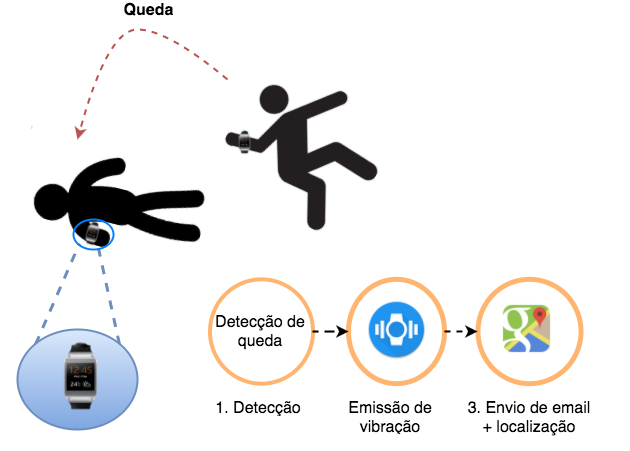
\includegraphics[scale=0.5]{imagens/DiagramaQueda.png}
	\caption{Aplicação no evento de queda. Figura Elaborada pelo autor (2016).}
	\label{fig:diagram}
\end{figure}



Assim que um evento de queda é detectado, o smartwatch irá emitir um sinal de vibração por um tempo determinado, e caso o usuário não informe o contrário, um email contendo a localização do usuário que está utilizando o smartwatch é enviado para os seus contatos de emergência previamente cadastrados.

O SafeWatch foi desenvolvido com base em uma arquitetura pré-definida e possui os seus módulos desacoplados para facilitar futuras mudanças ou melhorias. Na Figura \ref{fig:architecture} é possível ver o fluxo de dados dos cinco módulos presentes no SafeWatch. O fluxo começa com a obtenção dos dados do acelerômetro e termina com envio da mensagem de emergência. As setas na imagem representam o sentido do fluxo dos dados. Os módulos utilizados são os seguintes:


 \begin{figure}
 	\centering
 	\includegraphics[scale=0.65]{imagens/architecture.png}
 	\caption{ Fluxo de Dados do SafeWatch. Figura Elaborada pelo autor (2016).}
 	\label{fig:architecture}
 \end{figure} 


\begin{enumerate}
	\item{\textbf{Sensor Reader}: Responsável pela configuração e gerenciamento dos sensores, mais especificamente do sensor utilizado, o acelerômetro. }
	
	\item{\textbf{Fall Detector}: Recebe informações provindas do \textit{Sensor Reader} para através do algoritmo de detecção de quedas categorizar um determinado evento como queda ou não.}
	
	\item{\textbf{Watch Communicator}: Realiza a comunicação entre o smartwatch e o smartphone do usuário. Irá receber dados do smartwatch que são tratados pelo módulo chamado de \textit{Fall Handler}.}
	
	\item{\textbf{Fall Handler}: Será responsável pelas ações do smartphone após um evento de queda, como o envio de emails e o gerenciamento dos dados do acelerômetro recebidos do smartwatch.}
	
	\item{\textbf{Contact Manager}: Será responsável pelo gerenciamento dos contatos de emergência do usuário. Ações como visualização, adição e remoção de contatos estão encapsuladas neste módulo.}
			
\end{enumerate}

Os módulos \textit{Sensor Reader} e \textit{Fall Detector} estão presentes na aplicação embarcada no smartwatch, os demais módulos estão presentes na aplicação para smartphones. 



\section{Ferramentas Utilizadas}
\label{sec:tools}
Durante o desenvolvimento do \textit{SafeWatch} foram utilizadas diversas ferramentas que serviram para dar suporte a sua implementação e execução. Tanto o aplicativo para smartphones, quanto o aplicativo embarcado no smartwatch foram desenvolvidos utilizando o Android Studio\footnote{https://developer.android.com/studio/}. O Android Studio é a \ac{IDE} oficial do Google no desenvolvimento de aplicações móveis ou vestíveis.


Nas classes do projeto relacionadas às telas do aplicativo foi utilizado o ButterKnife\footnote{texthttps://github.com/JakeWharton/butterknife}. O ButterKnife é responsável por fazer a ligação entre os arquivos responsáveis pela criação das telas, e as classes que utilizam os componentes visuais destas telas. 

Para realizar os cálculos do desvio-padrão foi utilizada a biblioteca do Apache chamada Commons-Math\footnote{http://commons.apache.org/proper/commons-math/}. Esta biblioteca contém um conjunto de funções matemáticas e de estatística não presentes na biblioteca padrão do JAVA. 

Para que possamos enviar os dados do acelerômetro do smartwatch para o smartphone, eles precisam estar codificados em algum padrão, o padrão escolhido foi o JSON. O JSON é um formato de dados utilizado para comunicação entre dispositivos \citep{JSON16}. Para que possamos fazer a codificação e decodificação dos dados do acelerômetro foi utilizada a biblioteca chamada Gson\footnote{http://www.json.org/}.

Por fim, para o envio de emails para os contatos de emergência foi utilizada a biblioteca padrão criada pela Oracle\footnote{http://www.oracle.com/} chamada de JavaMail\footnote{http://www.oracle.com/technetwork/java/javamail/index.html}. 





\section{Implementação}
\label{sec:implementation}
A implementação do SafeWatch foi dividida em várias partes, onde cada uma delas é representada por um módulo independente dos demais. A linguagem de programação utilizada foi Java\footnote{http://www.oracle.com/technetwork/java/index.html}, linguagem padrão no desenvolvimento de aplicações Android. Nas seções a seguir são detalhados detalhes da implementação e funcionamento de cada módulo.


\subsection{Sensor Reader}
O módulo \textit{Sensor Reader} é responsável pela configuração e gerenciamento do acelerômetro. Aqui, o acelerômetro é configurado para atualizar seus dados a uma frequência de 50 $Hz$, ou seja, a cada 20 ms. Os dados do acelerômetro são coletados a todo momento, mesmo quando a aplicação não está em primeiro plano.

Este módulo também será responsável por armazenar os dados do acelerômetro nos últimos 0.4 segundos para posterior uso no algoritmo de detecção, caso necessário. Tanto a escolha da frequência de 50 $Hz$ quanto o tempo de 0.4 segundos para o armazenamento de dados do acelerômetro serão explicados com mais detalhes na Seção \ref{subsec:fall_detector}. 


\subsection{Fall Detector}
\label{subsec:fall_detector}
O módulo \textit{Fall Detector} encapsula o algoritmo de detecção de quedas baseado em limiares utilizado pelo SafeWatch. Este é o módulo mais complexo da aplicação, pois nele se encontra a lógica responsável por decidir, através dos dados obtidos do acelerômetro, se um evento de queda ocorreu ou não. O algoritmo proposto é uma adaptação do algoritmo desenvolvido por \cite{hsieh2014wrist}. 

O algoritmo proposto neste trabalho se diferencia do algoritmo proposto em \cite{hsieh2014wrist} pela não utilização do giroscópio como sensor auxiliar, pois acredita-se que sem o uso desse sensor é possível obter-se resultados satisfatórios, como visto na Seção \ref{subsec:hsieh}, reduzindo o custo de bateria. O giroscópio é usado por \cite{hsieh2014wrist} para aumentar o valor de \textit{Especificidade} do sistema proposto. Ele é utilizado como o primeiro passo no algoritmo baseado em limiares utilizado por ele. Nos experimentos realizados por \cite{hsieh2014wrist}, a velocidade angular obtida através do giroscópio possui valores maiores que 350º/s em um evento de queda. 

De acordo com um estudo feito por \cite{casilari2015analysis}, o número de sensores utilizados afeta diretamente a duração da bateria. Em um experimento realizado por \cite{mellone2012smartphone} utilizando um smartphone Samsung Galaxy S II, a duração da bateria aumentou de 16 para 30 horas ao utilizar somente um sensor (acelerômetro) em vez de três sensores (acelerômetro, magnetômetro, giroscópio). Além disso, o SafeWatch só utiliza um smartwatch, enquanto o sistema proposto por \cite{hsieh2014wrist} necessita de dois dispositivos de pulso similares a um smartwatch. 

Um grande desafio quando utilizamos um algoritmo baseado em limiares é a definição dos valores dos limiares. Caso esse valor seja muito alto, o sistema irá deixar escapar alguns eventos de queda, mas não irá categorizar uma \ac{AD} como uma queda.  Do outro lado, se esse valor for muito baixo, o sistema irá detectar todos os eventos de queda, mas algumas \ac{AD} pode ser categorizadas como eventos de queda de maneira equivocada. De acordo com o treinamento inicial realizado por \cite{hsieh2014wrist}, o valor de \ac{SMV}, representado pela fórmula \ref{eq:SMV}, será maior que $6G$, onde $G \approx 9.8 m/s^2$,  no momento do impacto em um evento de queda. 

Também foi identificado por \cite{hsieh2014wrist}, que caso o valor de aceleração atinja o valor de $6G$, o valor do desvio padrão ficava com valores em torno de $1.07G$  em movimentos regulares do braço realizados 0.4 segundos antes e depois deste pico de aceleração.Entretanto, em eventos de queda, este valor estava mais próximo de $1.69G$. 

Por fim, o período de inatividade posterior a uma queda foi analisado. De acordo com \cite{hsieh2014wrist}, o valor da \ac{SMA}, expresso através da Equação \ref{eq:SMA}, tem uma relação diretamente proporcional com o nível de movimentação de um corpo. Foi identificado que em eventos de queda, o indíviduo tende a ficar parado por pelo menos 2 segundos, com valores de SMA inferiores a $200G$. É importante ressaltar que este valor de $200G$ é encontrado quando a frequência do acelerômetro é de 50 $Hz$, ou seja, a cada $20 ms$ um novo valor do acelerômetro é coletado. Caso
está frequencia seja diferente, o número de amostra coletados será afetado, fazendo com que o valor de $SMA$ seja diferente de $200G$ em um periodo de inatividade.

\begin{equation}
SMA = \sum_{i=1}^{N} (\mid X_i\mid + \mid Y_i \mid + \mid Zi_i \mid)
\label{eq:SMA}
\end{equation}

Nesta equação $X_i$, $Y_i$, $Z_i$, são os valores da aceleração no tempo $i$ e $N$ é o número de amostras desejadas. Levando como base o treinamento inicial descrito acima foi possível desenvolver o algoritmo descrito na imagem \ref{fig:flow_chart}.

\begin{figure}[ht]
	\centering
	\includegraphics[scale=0.75]{imagens/flowChartAlgorithm.png}
	\caption{ Fluxograma do algoritmo proposto. Figura Elaborada pelo autor (2016).}
	\label{fig:flow_chart}
\end{figure} 

	\begin{enumerate}
		\item Os valores do acelerômetro são monitorados, caso $SMV$ seja maior do que $6G$, os demais valores de $SMV$ são monitorados por mais 0.4 segundos. O maior dos valores observado neste tempo é marcado como pico de aceleração e o algoritmo prossegue para o passo 2.
		\item O desvio padrão de \textit{SMV} é calculado, nos 0.4 segundos anteriores e posteriores a detecção do maior valor de SMV. Caso este valor não seja menor do que $1.5G$,  o algoritmo irá para o passo 3.
		\item O valor de $SMA$ é calculado, e caso este valor seja menor do que $ 200G $ finalmente confirmamos que um evento de queda ocorreu.
	\end{enumerate}

 
 
 Na figura \ref{fig:smartwatch_screen}, é possível ver os momento em que o sistema realiza a leitura de dados do acelerômetro, demonstrado pela tela da esquerda. Esta leitura é feita de maneira constante, mas não afeta o funcionamento das demais funções do smartwatch. 
 

 
 \begin{figure}[ht]
 	\centering
 	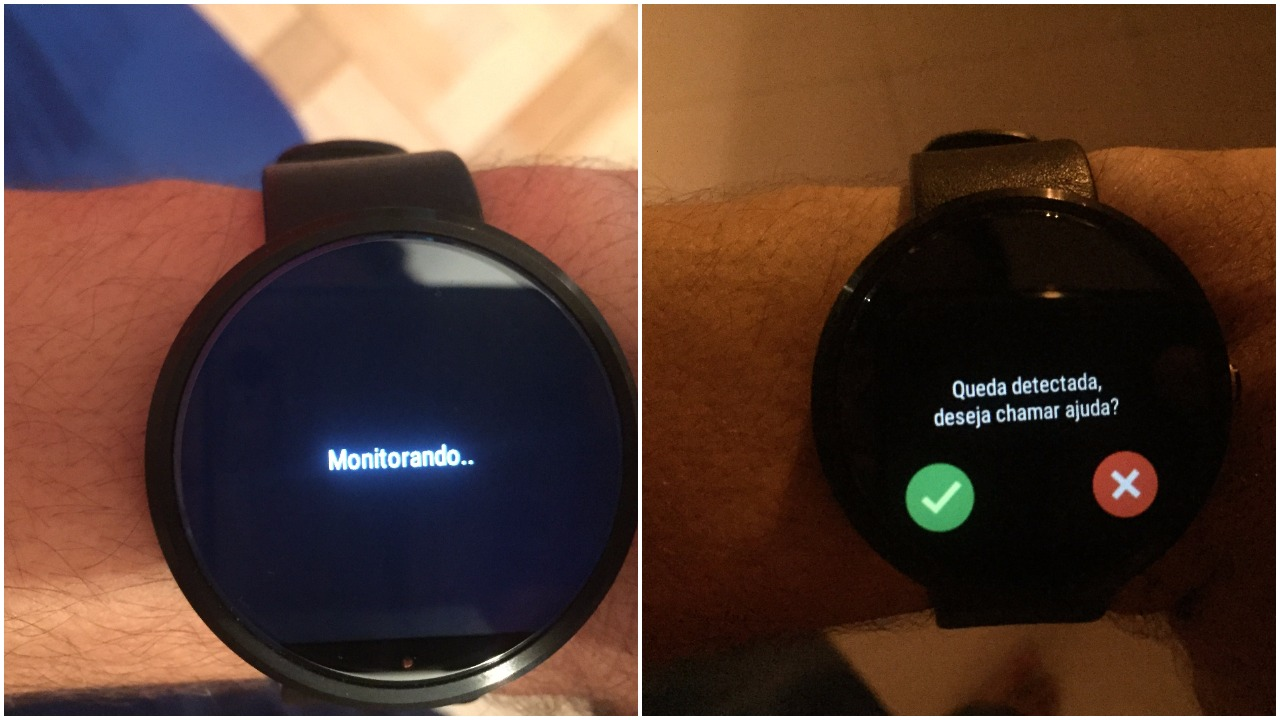
\includegraphics[scale=0.3]{imagens/smartwatch.png}
 	\caption{Na ordem, telas de monitoramento e detecção de quedas. Figura Elaborada pelo autor (2016).}
 	\label{fig:smartwatch_screen}
 \end{figure}
 
 O código fonte no apêndice \ref{ap:algorithm} representa o algoritmo utilizado para realizar a detecção de quedas implementado utilizado a linguagem de programação \textit{JAVA}. 

\subsection{Watch Communicator}
O módulo \textit{Watch Communicator} é responsável pela comunicação entre o smartwatch e o smartphone do usuário. Fisicamente, esta comunicação é realizada via bluetooth, já a nível de software, está comunicação é realizada através do que chamamos na arquitetura Android de \textit{Services}.

No Android, um \textit{Service} é um componente da aplicação capaz de realizar operações de longa duração em segundo plano \cite{servicesAndroidDocs}. No SafeWatch, os \textit{Services} recebem os dados do acelerômetro referentes ao evento de queda, ou seja, todos os registros do acelerômetro 0.4 segundos antes do pico de aceleração, até 2 segundos depois deste valor. Além disso, também é enviado, uma variável booleana indicando se deve-se ou não enviar um e-mail para a lista de contatos de emergência do usuário. Os emails de emergência são enviados para a lista de contato do usuário 15 segundos após um evento de queda, ou antes disso, caso o usuário confirme que precisa de ajuda. 

Para que os contatos da lista de emergência não sejam incomodados desnecessariamente na ocorrência de falsas detecções de quedas, o usuário poderá cancelar o envio dos emails de emergência, dentro de 15 segundos após um evento de queda, caso ele informe que está bem. O tempo de 15 segundos foi escolhido, pois o usuário terá tempo de dar um feedback para o sistema, caso ele não esteja em uma situação de perigo. Da mesma forma, este tempo não irá atrasar o envio da mensagem de emergência quando o usuário realmente precisar. Podemos ver a tela que aparecerá para o usuário em um evento de queda a direita na Figura \ref{fig:smartwatch_screen}. 



\subsection{Fall Handler} 
Este módulo é responsável pelo envio de e-mails e a manipulação de arquivos com os dados de uma queda. Para que se possa realizar o envio de e-mails, foi criado um email padrão do SafeWatch. O envio de e-mail é feito de forma assíncrona, sem bloquear a interação do usuário com a aplicação. O modelo do email pode ser visto na figura \ref{fig:mail_template}. Além de uma mensagem informando que o usuário pode está em uma situação de perigo, um link do \textit{Google Maps}\footnote{https://www.google.com/maps} é anexado com a última localização do usuário obtida pelo sistema.

\begin{figure}[ht]
	\centering
	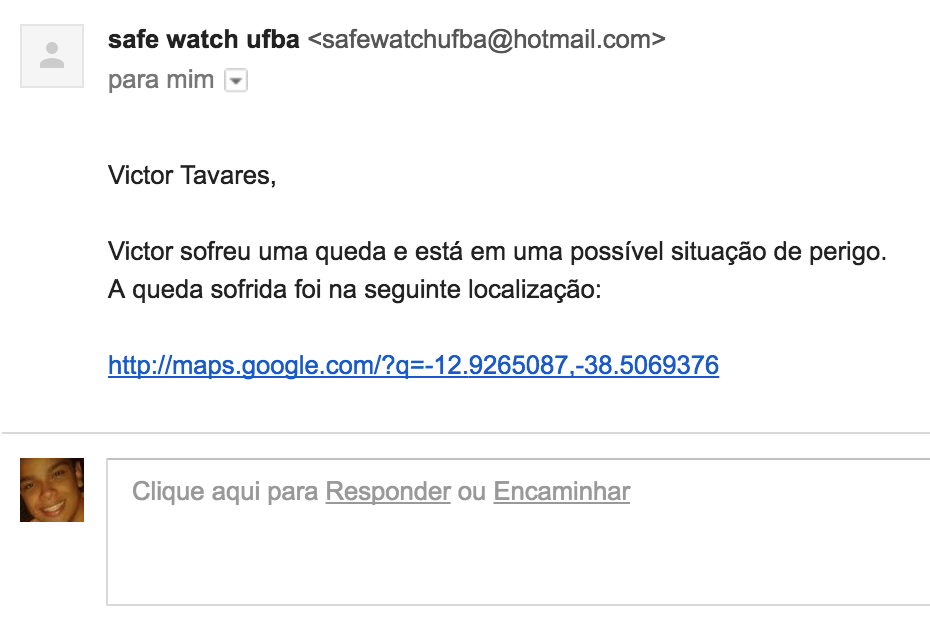
\includegraphics[scale=0.7]{imagens/mail_example.png}
	\caption{ Modelo de email enviado no evento de queda. Figura Elaborada pelo autor (2016).}
	\label{fig:mail_template}
\end{figure}


Os dados referentes a um evento de queda são salvos na raiz do sistema de arquivos do smartphone android na pasta \textit{/SafeWatch/smartwatch}. O arquivo é nomeado com o padrão \textit{experimentData\_timeStamp}, onde t\textit{timeStamp} representa o momento do salvamento do arquivo, em milisegundos. O arquivo está salvo no formato \textit{CSV}, com os valores de aceleração nos eixos x,y,z, o valor de \ac{SMV} correspondente ao registro e o tempo em milisegundos em que ele ocorreu. Apesar destes valores não serem úteis para o usuário final, eles poderão servir para uma possível análise dos dados de queda e replica dos experimentos realizados. 

\subsection{Contact Manager}
Neste módulo, estão encapsuladas as ações de adição, remoção e listagem dos contatos de emergência do usuário. O cadastro dos contatos de emergência deve ser a primeira ação do usuário no primeiro contato com a aplicação. A tela de cadastro e visualização dos contatos de emergência do usuário podem ser vistos na Figura \ref{fig:contacts}. Depois de adicionar os contatos de emergência, o usuário não necessita realizar mais nenhum tipo de cadastro ou configuração no sistema.


\begin{figure}
	\centering
	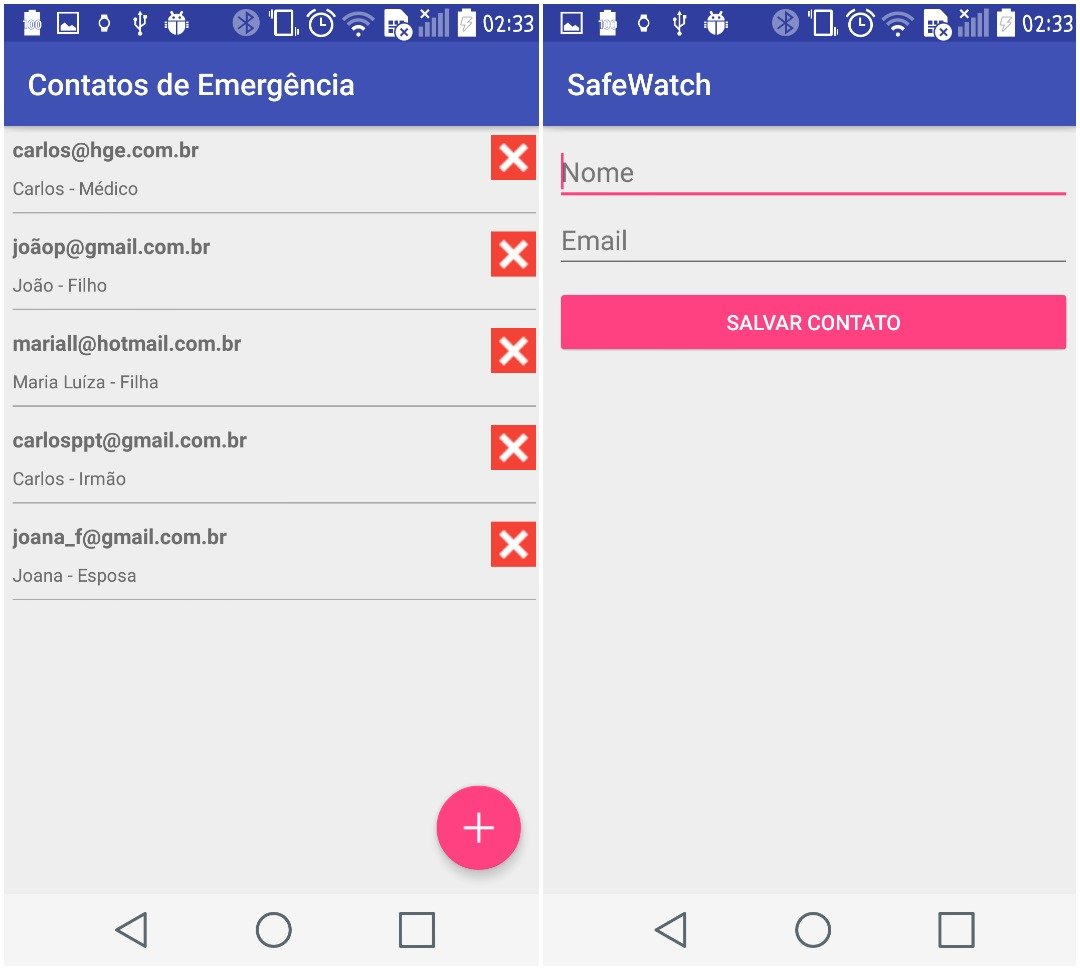
\includegraphics[scale=0.4]{imagens/add_list_contacts.png}
	\caption{Na ordem, telas de listagem e adição de contatos de emergência. Figura Elaborada pelo autor (2016).}
	\label{fig:contacts}
\end{figure}


\section{Sumário}
Neste capítulo foi apresentado uma visão geral do funcionamento do SafeWatch e as principais questões envolvidas no desenvolvimento deste trabalho. Foi descrito em detalhes o algoritmo de detecção de quedas utilizado e as telas presentes nesse sistema.  No próximo capítulo serão descritos detalhes do experimento e as métricas utilizadas na avaliação do SafeWatch. 



%\chapter{Estudo Experimental}
\label{cap:avaliacao}

Neste capítulo será apresentado o processo de avaliação utilizado para verificar a precisão do sistema de detecção de quedas proposto. Espera-se que o SafeWatch apresente uma precisão similar aos demais sistemas de detecção de quedas presentes na literatura.

As seções desse capítulo são organizadas da seguinte maneira: A Seção \ref{sec:metodology} apresenta os detalhes da metodologia utilizada para avaliar o SafeWatch; A Seção \ref{sec:metrics} mostra as métricas utilizadas na avaliação; A Seção \ref{sec:results} apresenta os resultados obtidos no experimento realizado e faz uma comparação com os resultados obtidos em outros trabalhos.



\section{Metodologia}
\label{sec:metodology}

Para avaliarmos o desempenho do SafeWatch foi realizado uma série de experimentos. O algoritmo de detecção de quedas proposto foi avaliado através de um conjunto de quedas simuladas e também um conjunto de atividades diárias realizadas pelos participantes do experimento. O grupo de voluntários possui um perfil diversificado, sendo composto de 3 homens e 5 mulheres como pode ser visto na Tabela \ref{tab:experiment}. O experimento não foi realizado com nenhum idoso devido a grande dificuldade de simular eventos de queda sem por em risco a integridade física do mesmo. Além disso, as base de dados encontradas referentes a eventos de quedas com idosos são privadas e não foram disponibilizadas, como vista no trabalho proposto por \cite{kostopoulos2015f2d}.


\begin{table}
	\centering
	\caption{Participantes do experimento}
	\label{tab:experiment}
	\begin{tabular}{c|c|c|c|c}
		\hline
		\textbf{Indivíduo}  & \textbf{Idade} 	& \textbf{Sexo}   &    \textbf{Peso}    & \textbf{Altura} 	 \\
		Indivíduo 1         &    28          & Masculino            & 82kg      		& 1.80m          \\  
		Indivíduo 2         &    20          & Feminino             & 63kg      		& 1.63m          \\
		Indivíduo 3         &    25          & Feminino             & 62kg      		& 1.59m          \\ 
		Indivíduo 4         &    29          & Masculino            & 130kg      		& 1.65m          \\ 
		Indivíduo 5         &    27          & Feminino             & 57kg      		& 1.69m          \\ 
		Indivíduo 6         &    14          & Feminino             & 45kg      		& 1.62m          \\
		Indivíduo 7         &    20          & Masculino            & 88kg      		& 1.80m          \\ 
		Indivíduo 8         &    30          & Feminino             & 62kg      		& 1.55m          \\   
	\end{tabular}
\end{table}

 
O smartwatch escolhido para realizar o experimento foi um \textit{Moto 360} da 1º geração com as seguintes características \citep{moto360}:

	\begin{enumerate}
		\item Sistema Operacional: Android Wear 2.0.
		\item CPU: Qualcomm Snapdragon 400, 1.2 GHz.
		\item Memória RAM: 512 MB.
		\item Capacidade de Armazenamento: 4 GB.
	\end{enumerate}
	
Já o smartphone escolhido foi um \textit{LG G2} com as seguintes características \citep{lg_g2}:

	\begin{enumerate}
		\item Sistema Operacional: Android  Lollipop 5.0.2.
		\item CPU: Quad-core 2.26 GHz Krait 400.
		\item Memória RAM: 2 GB.
		\item Capacidade de Armazenamento: 16GB.
	\end{enumerate}


Para avaliar o algoritmo de detecção de quedas implementado, foi realizado o seguinte experimento, composto de três etapas:

\begin{itemize}
	\item{\textbf{Preparação}: Nesta etapa é solicitado que o usuário coloque o smartwatch em seu pulso e ajuste a pulseira do relógio de uma maneira que o smartwatch permaneça firme, mas confortável. Depois disso, é informado que o usuário deverá simular duas quedas em cada um dos sentidos escolhidos: Costas, Frontal, Lado Direito, Lado Esquerdo. A ordem das quedas é decidida pelo usuário, o único requisito é que ele realize todas as oito quedas. }
	
	\item{\textbf{Realização das Quedas}: O usuário irá se posicionar de pé, na frente de um colchão coberto de almofadas como pode ser visto na Figura \ref{fig:fall_image}. A partir desta posição, ele irá realizar as oitos quedas, duas de cada tipo, como descrito na etapa anterior. A ordem das quedas é escolhida pelo usuário.  }
	
	\item{\textbf{Realização de Atividades Diárias}: Nesta etapa solicitamos que o usuário realize 4 atividades do seu cotidiano. Elas são: sentar em uma cadeira, levantar de uma cadeira, deitar no colchão e levantar do colchão. Estas atividades são realizadas afim de verificar se o sistema proposto é capaz de distinguir atividades diárias de um evento de queda. O sistema proposto não é capaz de distinguir qual a atividade diária que está sendo realizada, ele só é capaz de diferencia-la de um evento de queda.}
	
	
\end{itemize}


Além de executarem as simulações de queda antes das atividades diárias, ambos os eventos foram executados de maneira isolada, ou seja, não foi seguida nenhuma ordem ou sequência pré-definida de eventos. 

\begin{figure}[ht]
	\centering
	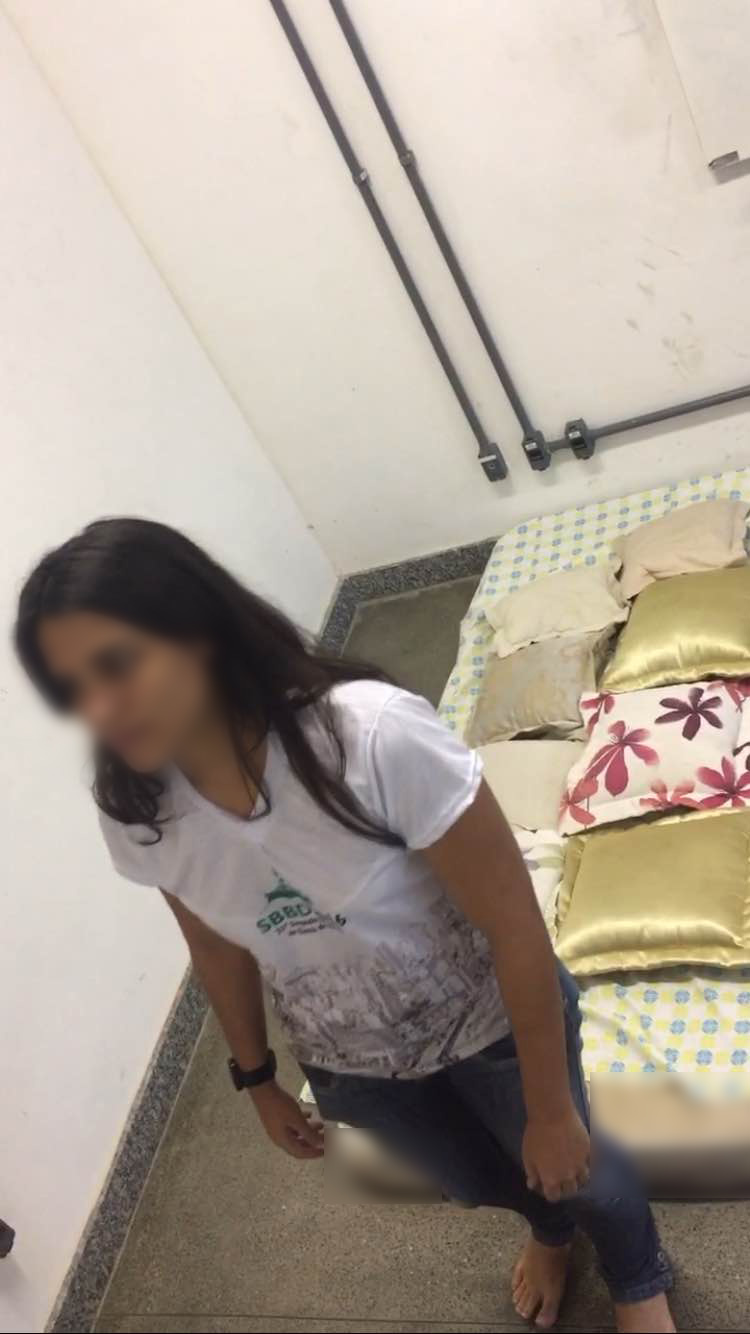
\includegraphics[scale=0.25]{imagens/fall_image.png}
	\caption{Usuário em preparação para uma queda de costas. Figura Elaborada pelo autor (2016).}
	\label{fig:fall_image}
\end{figure} 


\section{Métricas de Avaliação}
\label{sec:metrics}

Para que possamos analisar a performance do sistema de detecção de quedas foram utilizadas três métricas, a \textit{Sensibilidade},  \textit{Especificidade} e \textit{Acurácia}. De acordo com \cite{casilari2015automatic}, os valores de \textit{Sensibilidade} e \textit{Especificidade} são duas métricas bastante utilizadas na literatura para a análise de performance em sistemas de detecção de quedas. Elas representam, respectivamente, a proporção de eventos de queda e \ac{AD} que foram classificadas corretamente como tal. Já a \textit{Acurácia} é uma combinação da \textit{Sensibilidade} e da \textit{Especificidade} e nos dá uma ideia geral da performance do sistema.

A \textit{Sensibilidade} é expressa pela fórmula \ref{eq:Sensibilidade}. As variáveis \textit{TP} e \textit{FN} são, respectivamente, acrónimos para True Positive (Verdadeiro Positivo em inglês) e False Negative (Falso Negativo em inglês). A variável TP representa o número de eventos de queda corretamente classificadas, enquanto FN representa as quedas que não foram detectadas pelo sistema.

\begin{equation}
Sensibilidade = \frac{TP}{TP + FN}
\label{eq:Sensibilidade}
\end{equation}


Já a \textit{Especificidade} é expressa pela fórmula \ref{eq:Especificidade}. As variáveis \textit{TN} e \textit{FP} são, respectivamente acrónimos para True Negative (Verdadeiro Negativo em inglês) e False Positive (Falso Positivo em inglês). A variável TN representa o número de atividades diárias corretamente classificadas como tal, enquanto FP representa as atividades diárias que foram classificadas como queda.

\begin{equation}
Especificidade = \frac{TN}{FP + TN}
\label{eq:Especificidade}
\end{equation}

Para calcularmos a acurácia geral do sistema, devemos utilizar a fórmula \ref{eq:accuracy}. 

\begin{equation}
Acuracia = \frac{TP + TN}{TP + FP + TN + FN}
\label{eq:accuracy}
\end{equation}


\section{Resultados}
\label{sec:results}

Na tabela \ref{tab:results_fall} podemos ver os resultados dos experimentos de queda para cada um dos indivíduos. Como descrito na Seção \ref{sec:metodology} cada individuo realizou duas quedas em quatro sentidos diferente. Cada elemento da tabela representa o número de quedas que foram identificadas com sucesso pelo sistema em cada uma das direções. 

\begin{table}[h]
	\centering
	\caption{Resultados do experimentos de Queda.}
	\label{tab:results_fall}
	\begin{tabular}{c|c|c|c|c}
		\hline
		\textbf{Individuo}  & \textbf{Frente} 	& \textbf{Costas}   &    \textbf{Direita}    & \textbf{Esquerda} 	 \\
		Individuo 1         & 2        		    & 1            		& 2      		 		 & 2         \\  
		Individuo 2         & 1        		    & 2            		& 2      		 		 & 2         \\
		Individuo 3         & 2        		    & 2            		& 1      		 		 & 2         \\
		Individuo 4         & 2        		    & 2            		& 2      		 		 & 2         \\
		Individuo 5         & 2        		    & 1            		& 2      		 		 & 1         \\
		Individuo 6         & 2        		    & 2            		& 2      		 		 & 1         \\
		Individuo 7         & 2        		    & 2            		& 2      		 		 & 2         \\
		Individuo 8         & 2        		    & 1            		& 2      		 		 & 2         \\
	\end{tabular}
\end{table}


Como podemos ver na tabela \ref{tab:results_fall}, o número de verdadeiros-positivos é de 57, enquanto o número de falsos-negativos é de somente 7, o que nos dá uma \textit{especificidade} de $89,06\%$. Foi possível observar que o limiar inicial de $6G$ no algoritmo de detecção de quedas não foi alcançado em todos os eventos erroneamente não categorizados como queda.


Já na tabela \ref{tab:results_adl}, podemos ver os resultados do experimentos de \ac{AD} para cada um dos indivíduos. Cada um deles realizou quatro tipos de \ac{AD}, como descrito na Seção \ref{sec:metodology}. Cada elemento da tabela representa o número de \ac{AD} que não foram identificadas pelo sistema como um evento de queda. 


\begin{table}[h]
	\centering
	\caption{Resultados do experimentos de Atividades Diárias.}
	\label{tab:results_adl}
	\begin{tabular}{c|c|c|c|c}
		\hline
		\textbf{Individuo}  & \textbf{Levantar(Cadeira)} 	& \textbf{Sentar(Cadeira)}   &    \textbf{Levantar(Cama)}    & \textbf{Deitar(Cama)} 	 \\
		Individuo 1         & 2        		    & 2            		& 2      		 		 & 2         \\  
		Individuo 2         & 2        		    & 2            		& 2      		 		 & 2         \\
		Individuo 3         & 2        		    & 2            		& 2      		 		 & 2         \\
		Individuo 4         & 2        		    & 2            		& 2      		 		 & 2         \\
		Individuo 5         & 2        		    & 2            		& 2      		 		 & 2         \\
		Individuo 6         & 2        		    & 2            		& 2      		 		 & 2         \\
		Individuo 7         & 2        		    & 2            		& 2      		 		 & 2         \\
		Individuo 8         & 2        		    & 2            		& 2      		 		 & 2         \\
	\end{tabular}
\end{table}

 

Neste experimento, nenhum dos 64 eventos \ac{AD} foi identificado como um evento de queda pelo sistema, levando a uma \textit{especificidade} de $100\%$. De forma geral o sistema possui uma \textit{acurácia} de $94,53\%$.


Como visto na Tabela \ref{tab:compare}, o algoritmo proposto neste trabalho apresentou resultados satisfatórios identificando um evento de queda em quase $90\%$ dos casos, e não apresentando nenhum falso-positivo nas \ac{AD} testadas. Em comparação com o Speedy, sistema desenvolvido por \cite{degen2003speedy}, o nosso sistema apresentou uma sensibilidade $24,06\%$ maior, ou seja, o SafeWatch apresentou uma especificidade de $89,06\%$ contra $65\%$ do Speedy em experimentos bastantes similares.

\begin{table}[h]
	\centering
	\caption{Comparação com os resultados dos Trabalhos Relacionados.}
	\label{tab:compare}
	\begin{tabular}{c|c|c|c|c}
		\hline
		\textbf{}  & \textbf{SafeWatch} 	& \textbf{Speedy}   &    \textbf{F2D}    & \textbf{Sistema de Detecção de Pulso} 	 \\
		Sensibilidade         & 89,06\%        		    & 65\%           & 93,48\%      		 		 & 95\%         \\  
		Especificidade        & 100\%        		    & -           	 & 98,54\%      		 		 & 96,07\%         \\
		Acurácia        	  & 94,53\%        		    & -              & 96,01\%      		 		 & 95,85\%         \\

	\end{tabular}
\end{table}

Entretanto em comparação com \cite{hsieh2014wrist}, este trabalho apresentou uma \textit{sensibilidade} $5,94\%$ menor e uma \textit{especificidade} $3,3\%$ maior. Um dos prováveis motivos desse valor menor de \textit{Sensibilidade} são as condições do experimento.  Os experimentos realizados por \cite{hsieh2014wrist} foram em uma superfície acolchoada mais fina que um colchão convencional, o que leva a uma aceleração maior no impacto, podendo diminuir o número de falsos-negativos no experimento realizado. Em relação ao tipos de quedas realizados, tanto este, quanto o trabalho proposto por \cite{hsieh2014wrist} apresentaram quatro tipos de quedas: frontais, laterais (Direito e Esquerdo), Costas. Já em relação as \ac{AD}, ele apresentou um número maior de atividades, incluindo andar e correr, o que pode levar a número maior de falso-positivos. 









\bibliographystyle{natbib}
\addcontentsline{toc}{chapter}{\bibliographytocname}
\bibliography{references}

% Appendix
%\clearpage
%\addappheadtotoc
%\appendix
%\appendixpage
%\chapter{Formulário}
\label{ap:formulario}


\def \tick{
$[$\hspace{0.3cm}$]$
}

\def \twooption#1#2{
\tick #1.  \tick #2.
}

\def \threeoption#1#2#3{
\tick #1.\newline
\tick #2.\newline
\tick #3.
}

\def \fouroption#1#2#3#4{
\tick #1.\newline
\tick #2.\newline
\tick #3.\newline
\tick #4.
}

\def \fiveoption#1#2#3#4#5{
\tick #1.\newline
\tick #2.\newline
\tick #3.\newline
\tick #4.\newline
\tick #5.
}
\def \datefield{
%date fied used in time sheets
    /\hspace{0.4cm}/
}

\def \rcolor{
%table row color
    \rowcolor[gray]{0.9}
}

\def \hcolor{
    \rowcolor[gray]{0.7}
}


\section{Formulário para o usuário do NLP Discovery}
\label{ap:sec:feedback}

\textbf{Nome: }
\\
\line(1,0){380}
\\
\textbf{Você tem algum conhecimento técnico a respeito de Serviços Web? }
\\
\twooption{Sim}{Não}
\\
\textbf{Encontrou alguma dificuldade ao utilizar a ferramenta?}
\\
\twooption{Sim}{Não}
\\
\textbf{Caso tenha respondido "Sim", detalhe a dificuldade encontrada:}
\\
\line(1,0){410}
\\
\line(1,0){410}
\\
\line(1,0){410}
\\
\line(1,0){410}
\\
\textbf{Qual foi a consulta realizada na ferramenta (Digite exatamente o mesmo texto que digitou na caixa de pesquisa da ferramenta)?  }
\\
\line(1,0){410}
\\
\line(1,0){410}
\\
\line(1,0){410}
\\
\line(1,0){410}
\\
\textbf{A busca gerou algum resultado relevante?}
\\
\twooption{Sim}{Não}
\\
\textbf{Caso tenha respondido "Sim", qual a posição do Serviço relevante no resultado?}
\\
\line(1,0){100}
\\


\end{document}